%%%%%%%%%%%%%%%%%%%%%%%%%%%%%%%%%%%%%%%%%
% Beamer Presentation
% LaTeX Template
% Version 1.0 (01/07/19)
%
%%%%%%%%%%%%%%%%%%%%%%%%%%%%%%%%%%%%%%%%%

%---------------------------------------------------------------------------------------------------------------------------------------------------
%	PACKAGES AND THEMES                                                           -------------------------------------------------------------------------
%---------------------------------------------------------------------------------------------------------------------------------------------------

\documentclass{beamer}

\mode<presentation> {

\usetheme{Frankfurt}
\usecolortheme{dove}

}

\usepackage{graphicx}
\usepackage{booktabs} 
%\usepackage{subfig}
\usepackage{pgf}
\usepackage{multirow}
\usepackage{appendixnumberbeamer}
\usepackage{subcaption}


%---------------------------------------------------------------------------------------------------------------------------------------------------
%	GENERAL OPTIONS                                                                     -------------------------------------------------------------------------
%---------------------------------------------------------------------------------------------------------------------------------------------------

% Set template options
\setbeamertemplate{section in toc}{\inserttocsectionnumber.~\inserttocsection}
\setbeamertemplate{frametitle}{\vspace*{1em}\insertframetitle}
\setbeamertemplate{enumerate items}[default]
\setbeamercolor{section in head/foot}{fg=white, bg=black}

% Headline
\makeatletter
\setbeamertemplate{headline}
{%
  \pgfuseshading{beamer@barshade}%
    \vskip-5ex%
  \begin{beamercolorbox}[ignorebg,ht=2.25ex,dp=3.75ex]{section in head/foot}
  \insertsectionnavigationhorizontal{\paperwidth}{\hskip0pt plus1fill}{\hskip0pt plus1fill}
  \end{beamercolorbox}%
  \ifbeamer@sb@subsection%
    \begin{beamercolorbox}[ignorebg,ht=2.125ex,dp=1.125ex,%
      leftskip=.3cm,rightskip=.3cm plus1fil]{subsection in head/foot}
      \usebeamerfont{subsection in head/foot}\insertsubsectionhead
    \end{beamercolorbox}%
  \fi%
}%
\makeatother

% Footline
\makeatletter
\setbeamertemplate{footline}
{
  \leavevmode%
  \hbox{%
  \begin{beamercolorbox}[wd=.333333\paperwidth,ht=2.25ex,dp=1ex,left]{section in head/foot}%
    \usebeamerfont{author in head/foot}\hspace{10pt}\insertshortauthor
  \end{beamercolorbox}%
  \begin{beamercolorbox}[wd=.333333\paperwidth,ht=2.25ex,dp=1ex,center]{section in head/foot}%
    \usebeamerfont{title in head/foot}\insertshorttitle
  \end{beamercolorbox}%
  \begin{beamercolorbox}[wd=.333333\paperwidth,ht=2.25ex,dp=1ex,right]{section in head/foot}%
    \usebeamerfont{date in head/foot}\insertshortdate{}\hspace*{2em}
    \insertframenumber{}\hspace*{2em}
  \end{beamercolorbox}}%
  \vskip0pt%
}
\makeatother

% Add logo
\logo{\pgfputat{\pgfxy(0,7)}{
\includegraphics[width=0.1\paperwidth]{Pictures/Unibe_Logo}}}

% Table settings
\renewcommand{\arraystretch}{2}
\captionsetup{labelformat=empty,labelsep=none}


%---------------------------------------------------------------------------------------------------------------------------------------------------
%	TITLE PAGE                                                                                    -------------------------------------------------------------------------
%---------------------------------------------------------------------------------------------------------------------------------------------------

\title[FEA II - The FEniCS Project]{
\LARGE
\uppercase{FINITE ELEMENT ANALYSIS II} \\ 
\normalsize Modelization of hyperelastic behavior of the brain
} 

\author{Mathieu Simon}
\institute[University of Bern]
{
MSc - Biomedical Engineering \\
University of Bern, Faculty of Medicine \\
\medskip
}
\date{June 19, 2020}

\begin{document}

\begin{frame}
\titlepage
\end{frame}

\begin{frame}
\frametitle{Overview}
\tableofcontents 
\end{frame}


%---------------------------------------------------------------------------------------------------------------------------------------------------
%	PRESENTATION SLIDES                                                              -------------------------------------------------------------------------
%---------------------------------------------------------------------------------------------------------------------------------------------------

%---------------------------------------------------------------------------------------------------------------------------------------------------
%---------------------------------------------------------------------------------------------------------------------------------------------------
%---------------------------------------------------------------------------------------------------------------------------------------------------
\section{FE vs Analytic - Comparative Plots}

\subsection{Incompressible Models}
\begin{frame}
\frametitle{Incompressible Models}
\begin{columns}[c] 
\column{.1\textwidth}
\hspace{4mm}
\rotatebox{90}{\hspace{5mm} Zoom\hspace{15mm} General}
\column{1\textwidth}
\begin{figure}
\hspace{-9mm}
\captionsetup[subfigure]{labelformat=empty}
\subfloat[]{
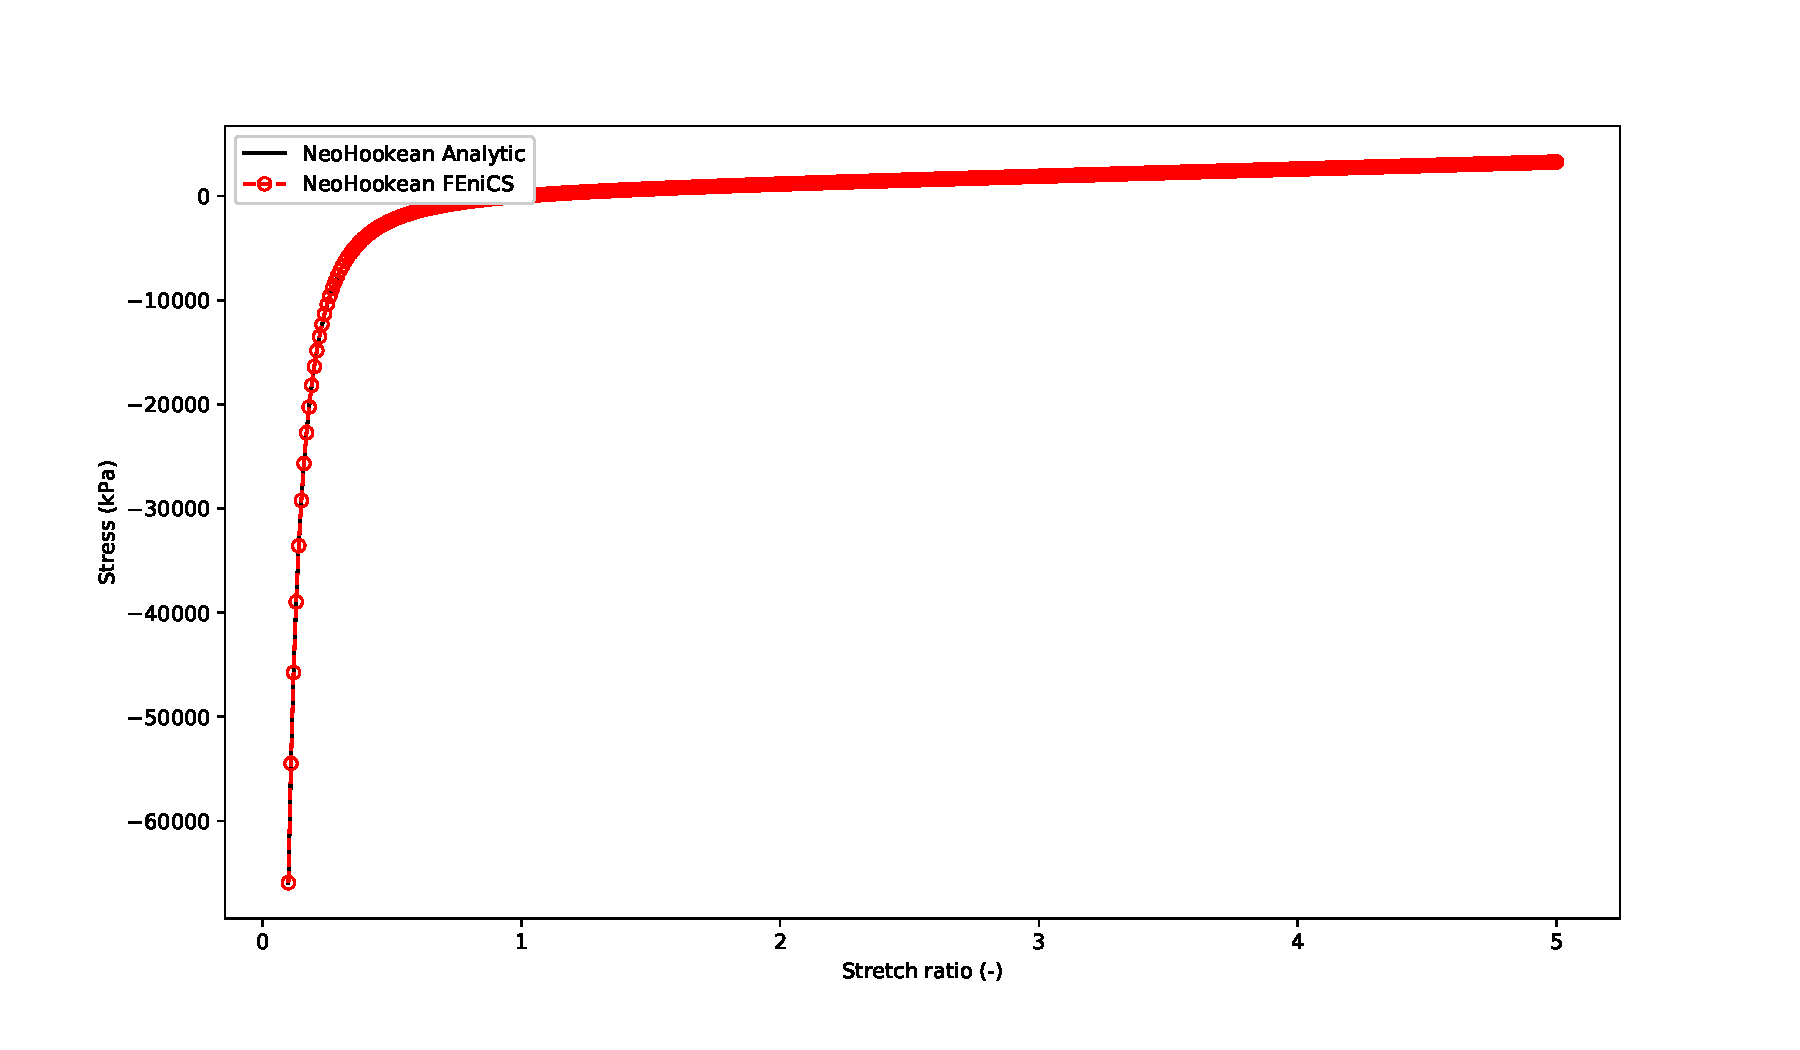
\includegraphics[width=0.25\linewidth, trim =  125 0 125 0]
{Pictures/NeoHookeanIncompressibleComparison}}
\qquad
\subfloat[]{
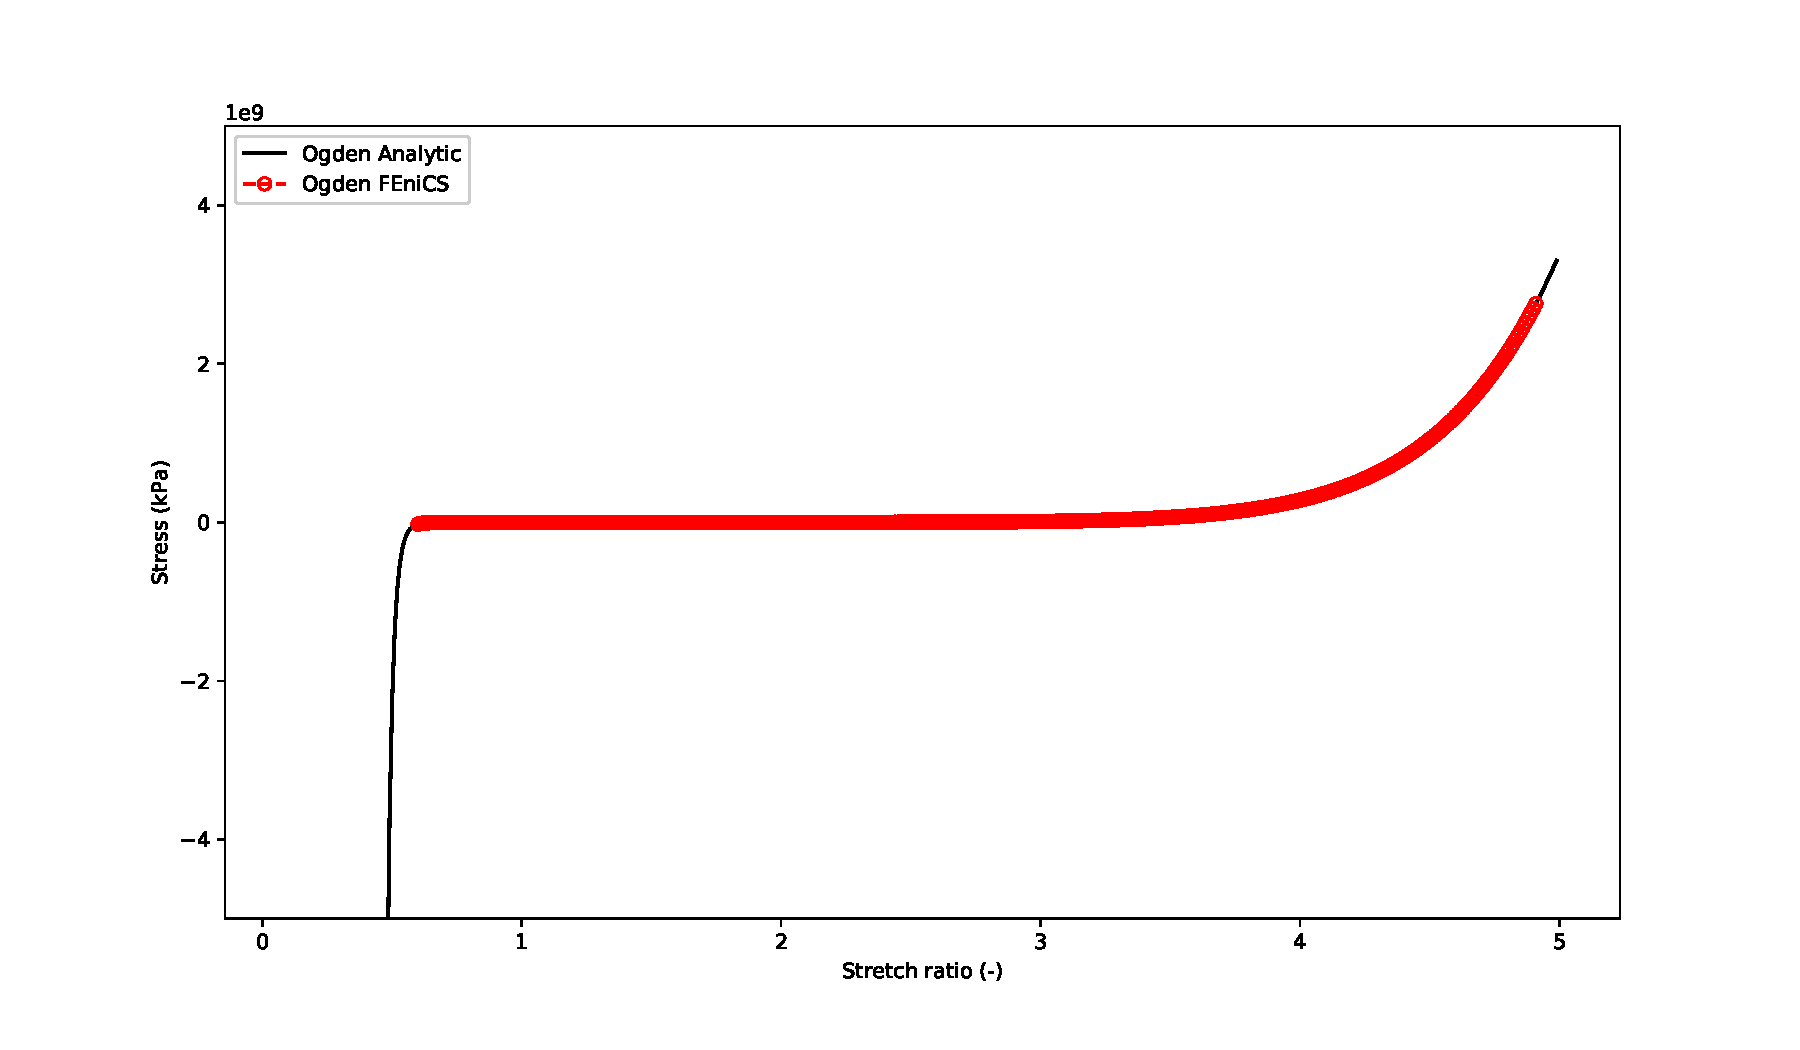
\includegraphics[width=0.25\linewidth, trim =  125 0 125 0]
{Pictures/OgdenIncompressibleComparison}}
\qquad
\subfloat[]{
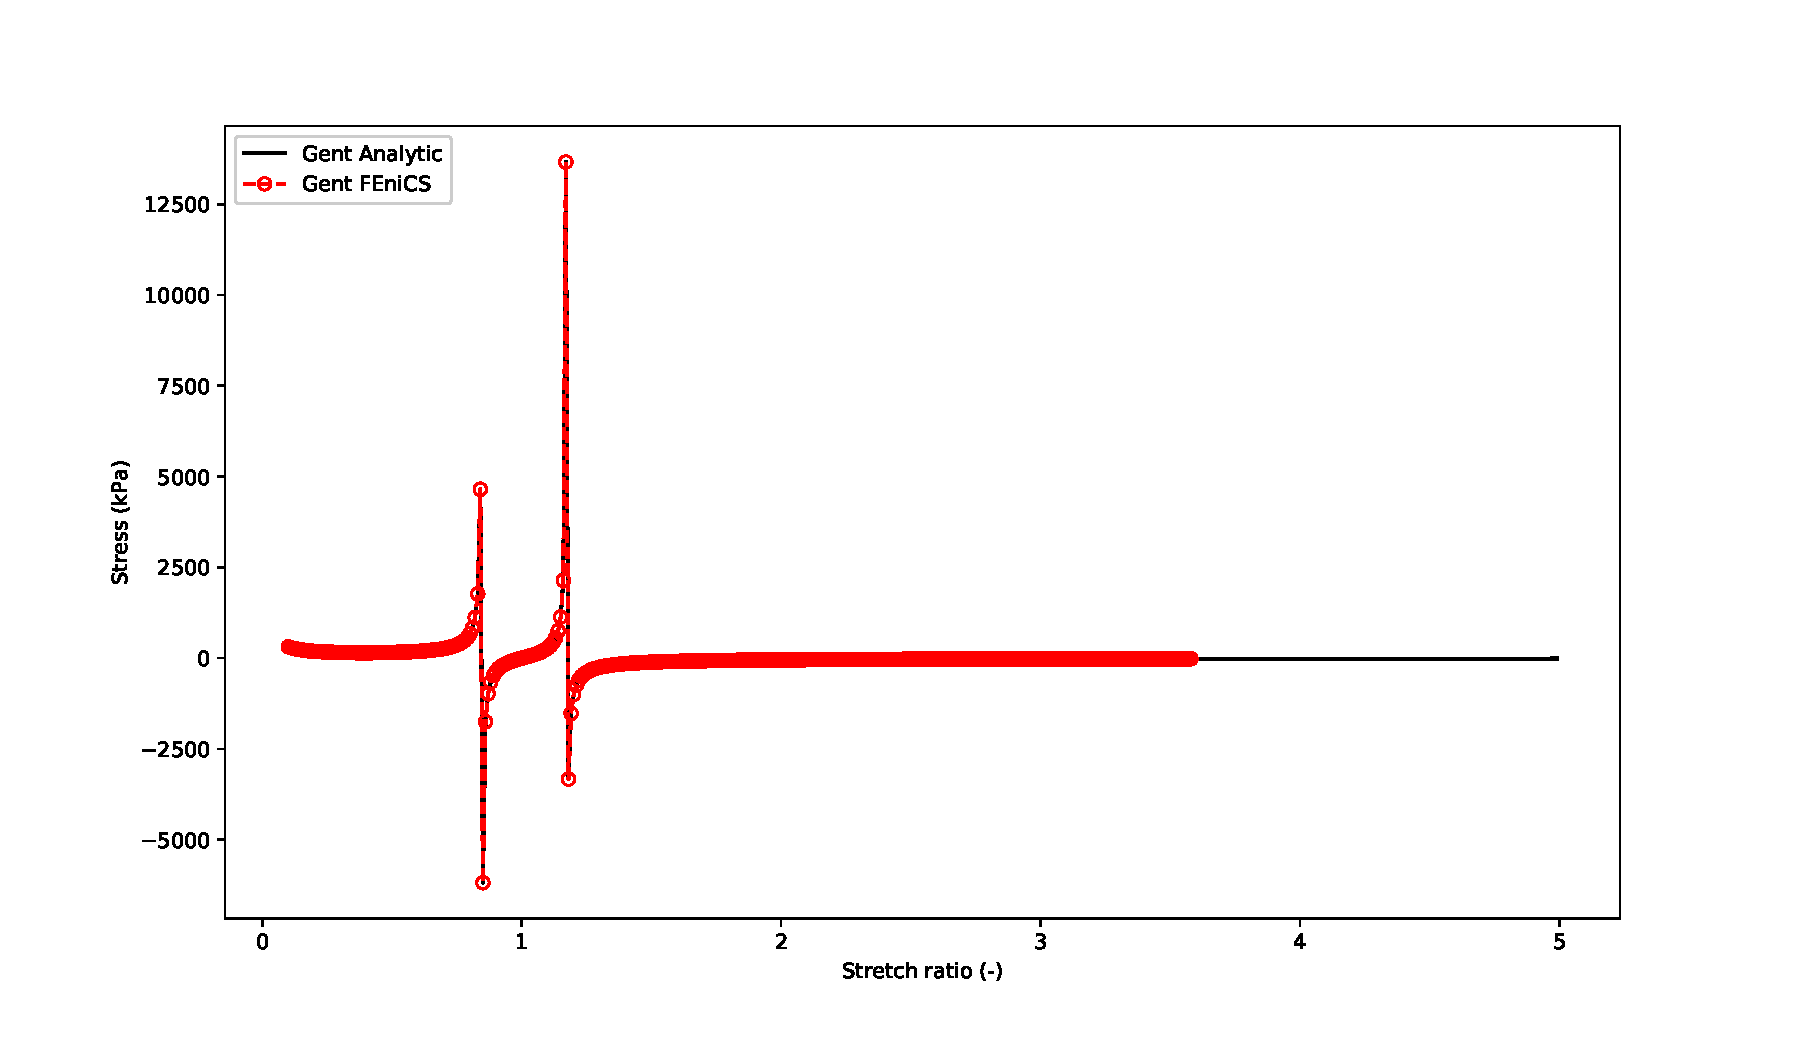
\includegraphics[width=0.25\linewidth, trim =  125 0 125 0]
{Pictures/GentIncompressibleComparison}}
\qquad
\subfloat[Neo-Hookean]{
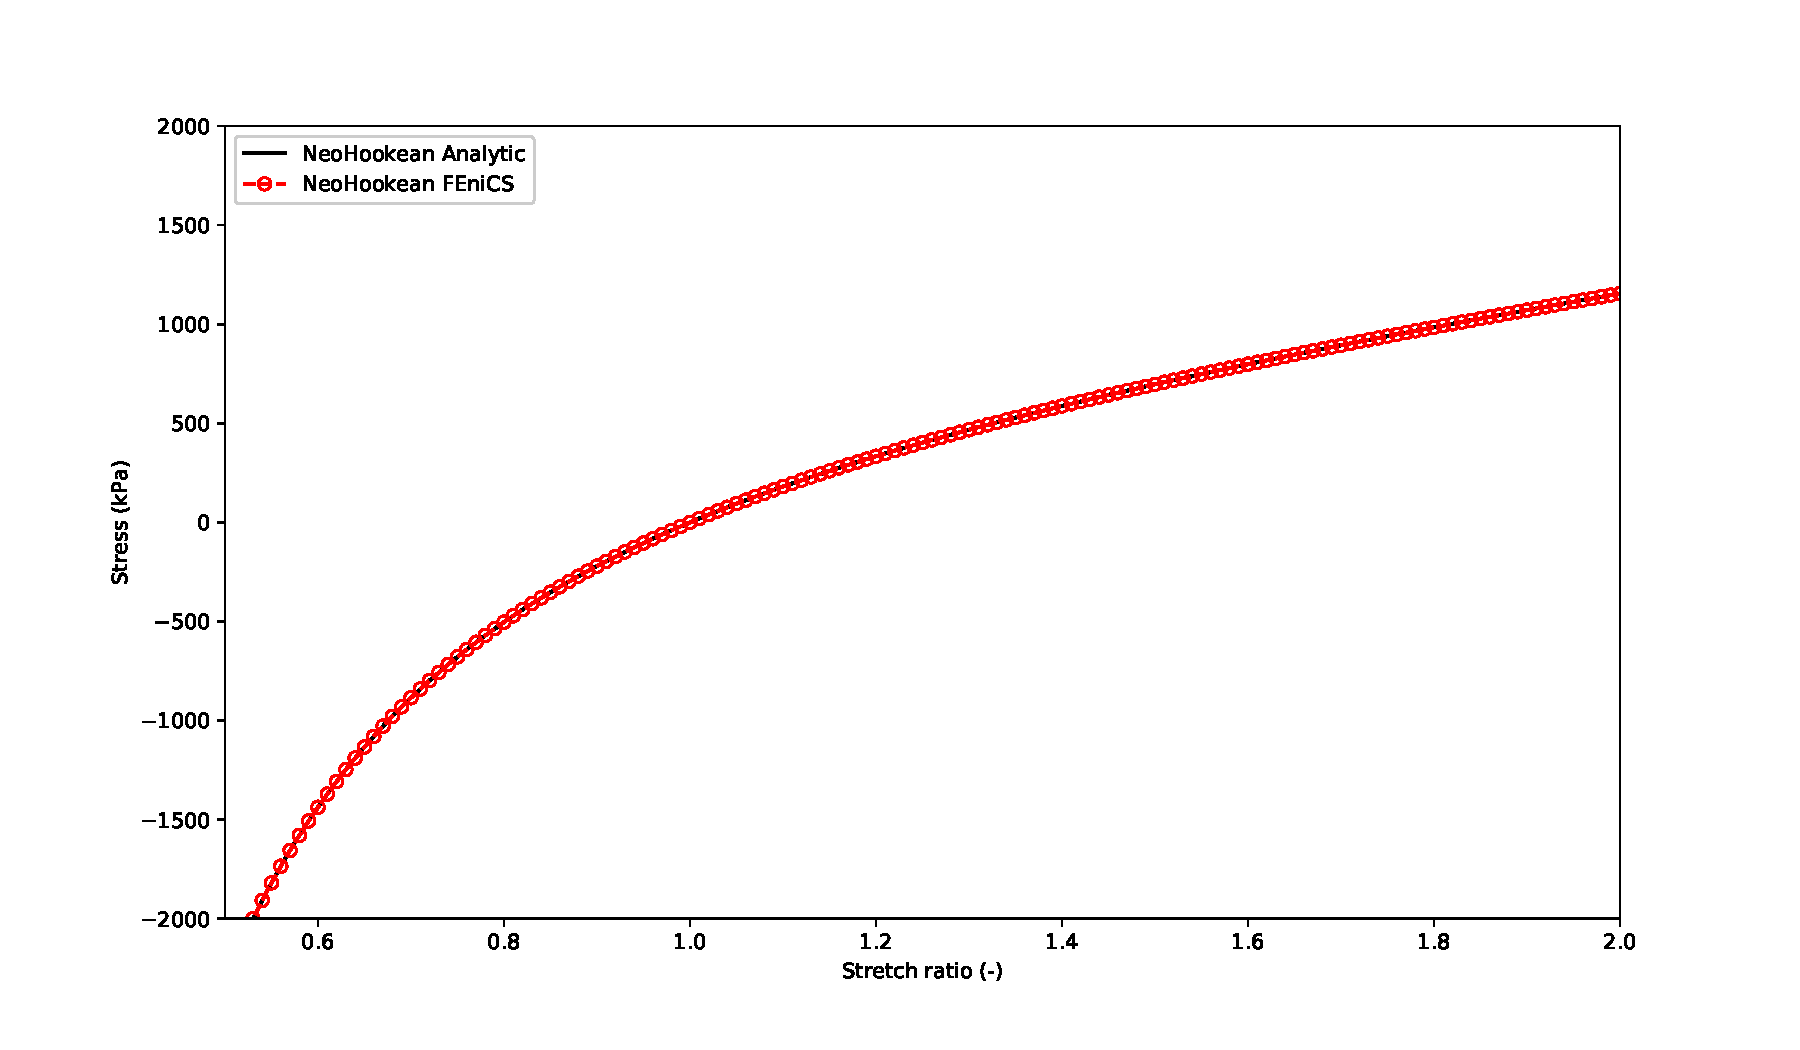
\includegraphics[width=0.25\linewidth, trim = 125 0 125 0]
{Pictures/NeoHookeanIncompressibleComparisonZoom}}
\qquad
\subfloat[Ogden]{
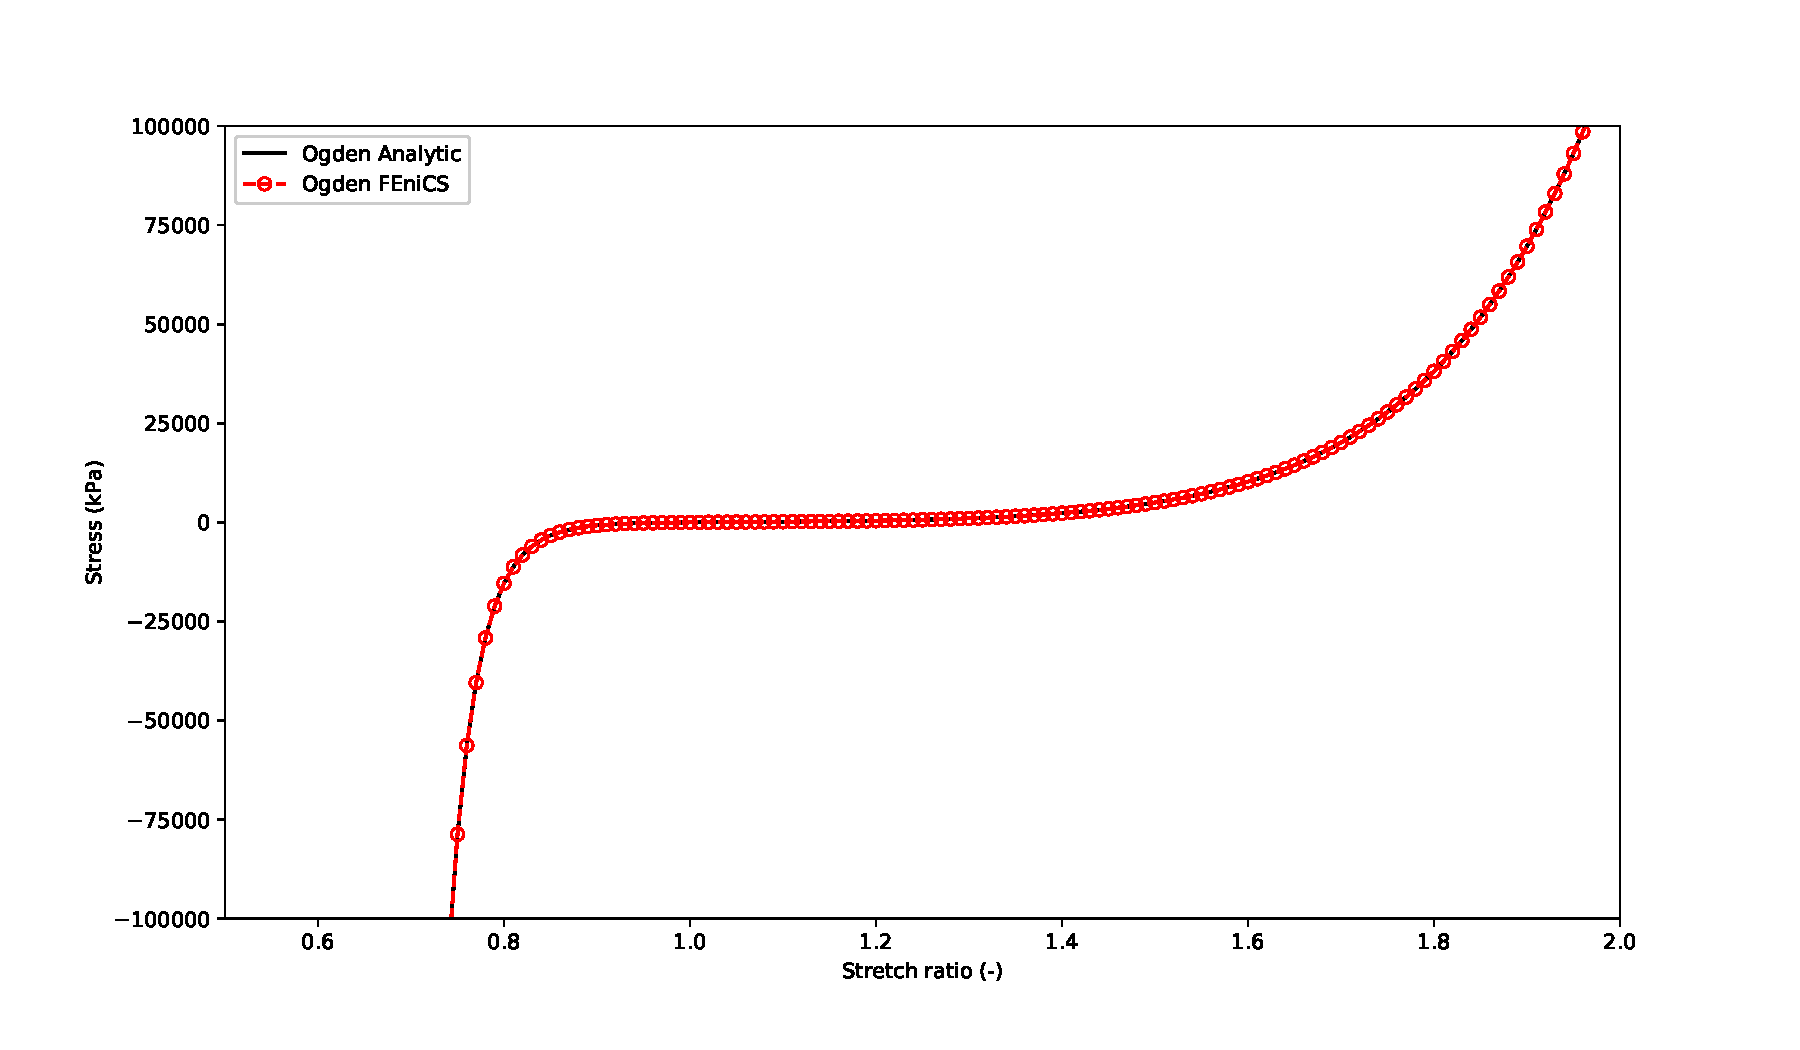
\includegraphics[width=0.25\linewidth, trim = 125 0 125 0]
{Pictures/OgdenIncompressibleComparisonZoom}}
\qquad
\subfloat[Gent]{
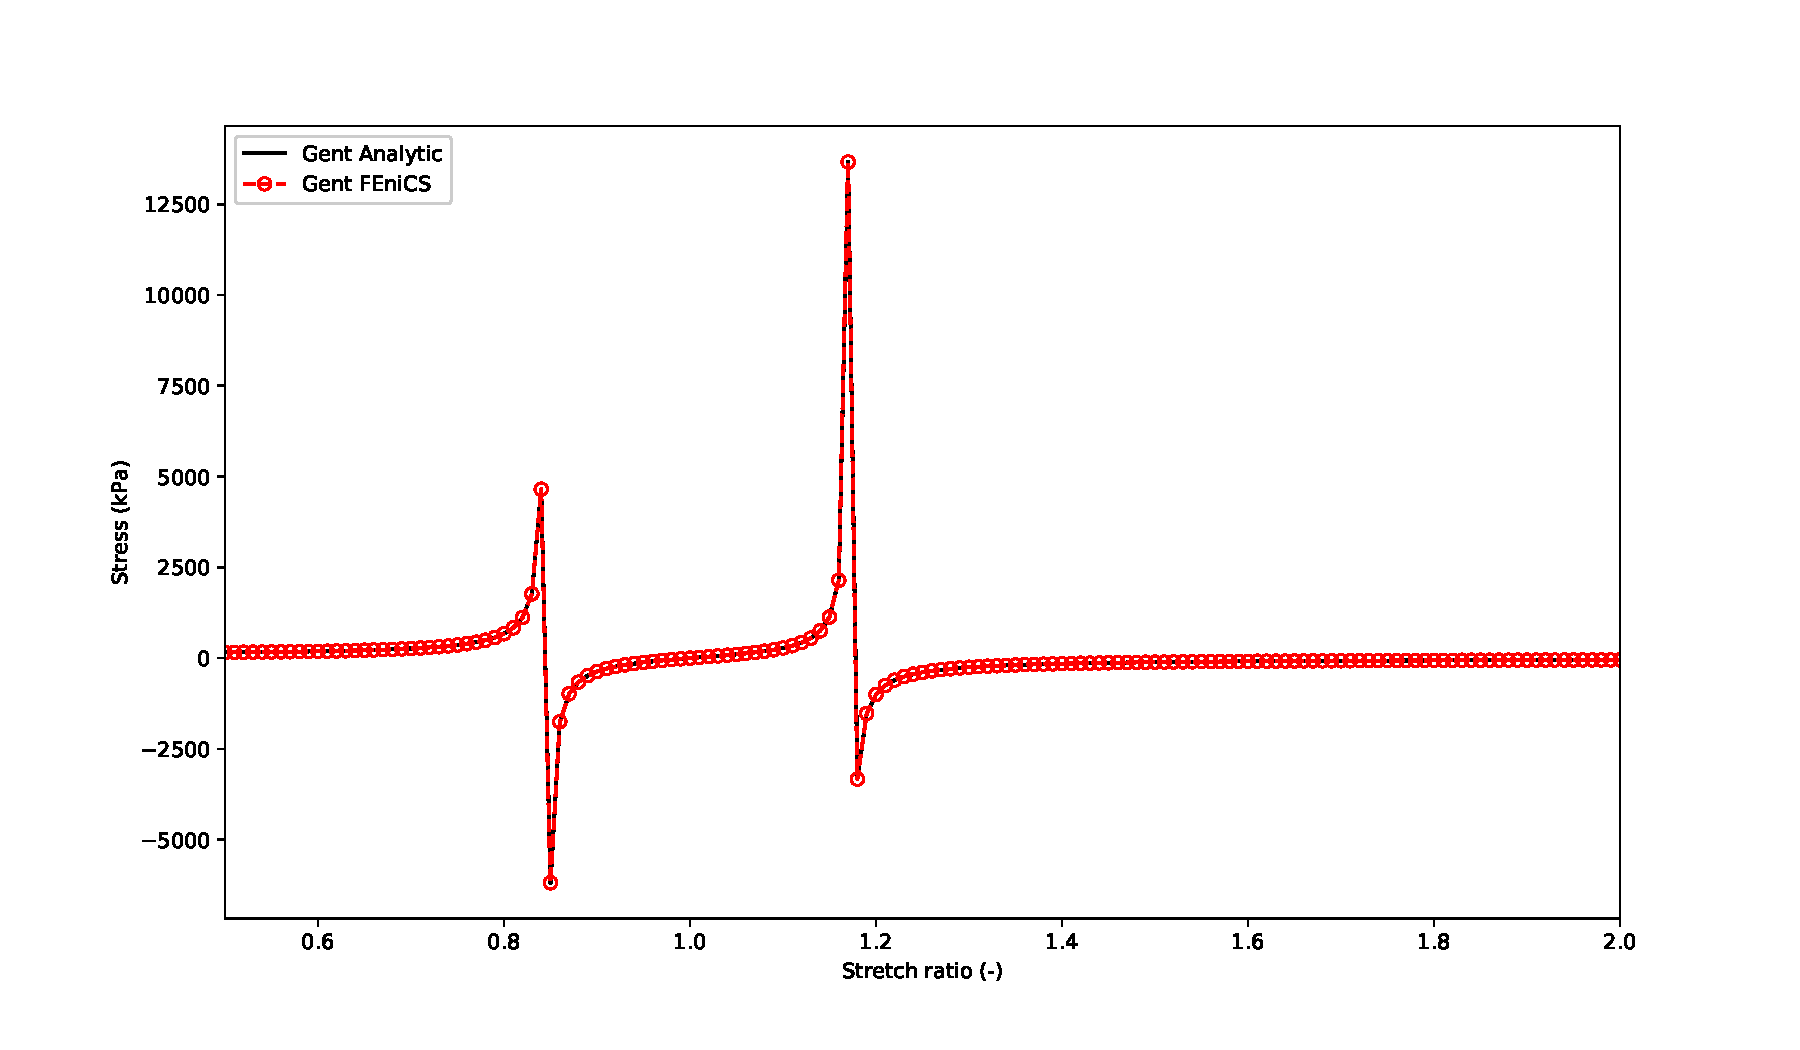
\includegraphics[width=0.25\linewidth, trim = 125 0 125 0]
{Pictures/GentIncompressibleComparisonZoom}}\hspace{7mm}
\end{figure}
\vfill
\end{columns}
\end{frame}

\subsection{Compressible Models}
\begin{frame}
\frametitle{Compressible Models}
\begin{columns}[c] 
\column{.1\textwidth}
\hspace{4mm}
\rotatebox{90}{\hspace{5mm} Zoom\hspace{15mm} General}
\column{1\textwidth}
\begin{figure}
\hspace{-0mm}
\captionsetup[subfigure]{labelformat=empty}
\subfloat[]{
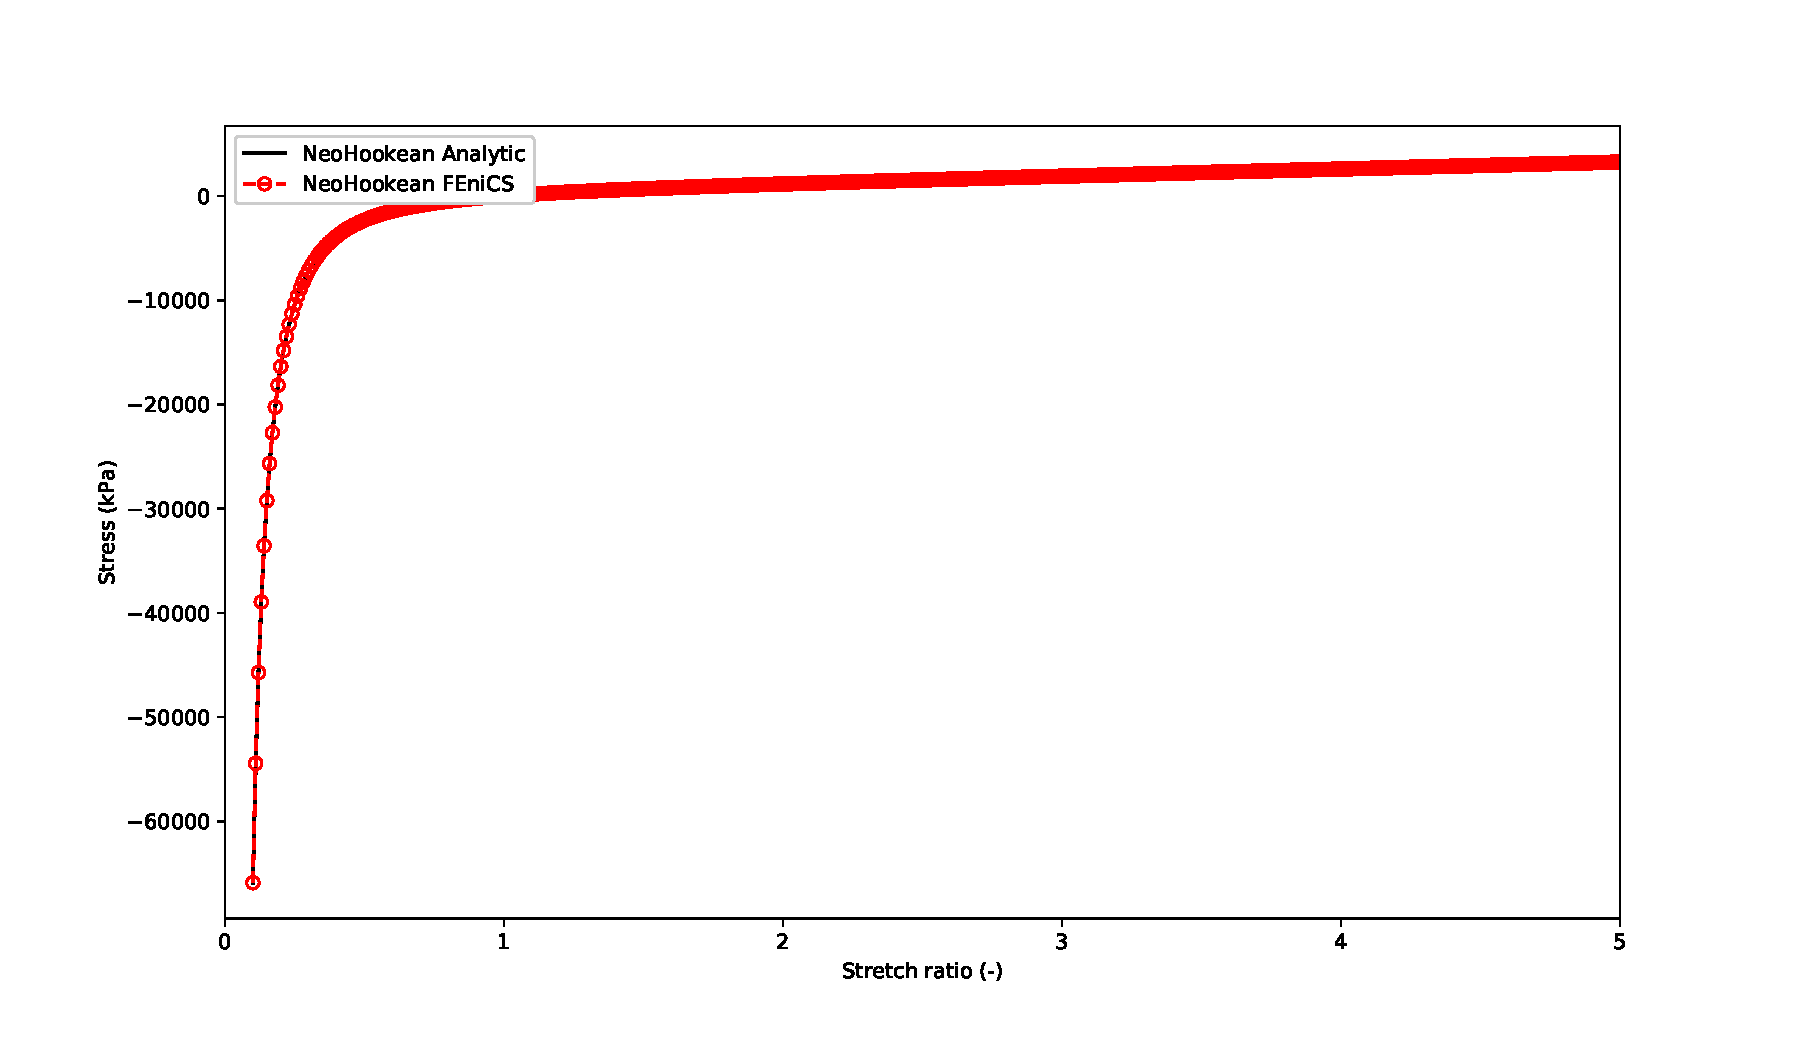
\includegraphics[width=0.25\linewidth, trim =  125 0 125 0]
{Pictures/NeoHookeanCompressibleComparison}}
\hspace{25mm}
\subfloat[]{
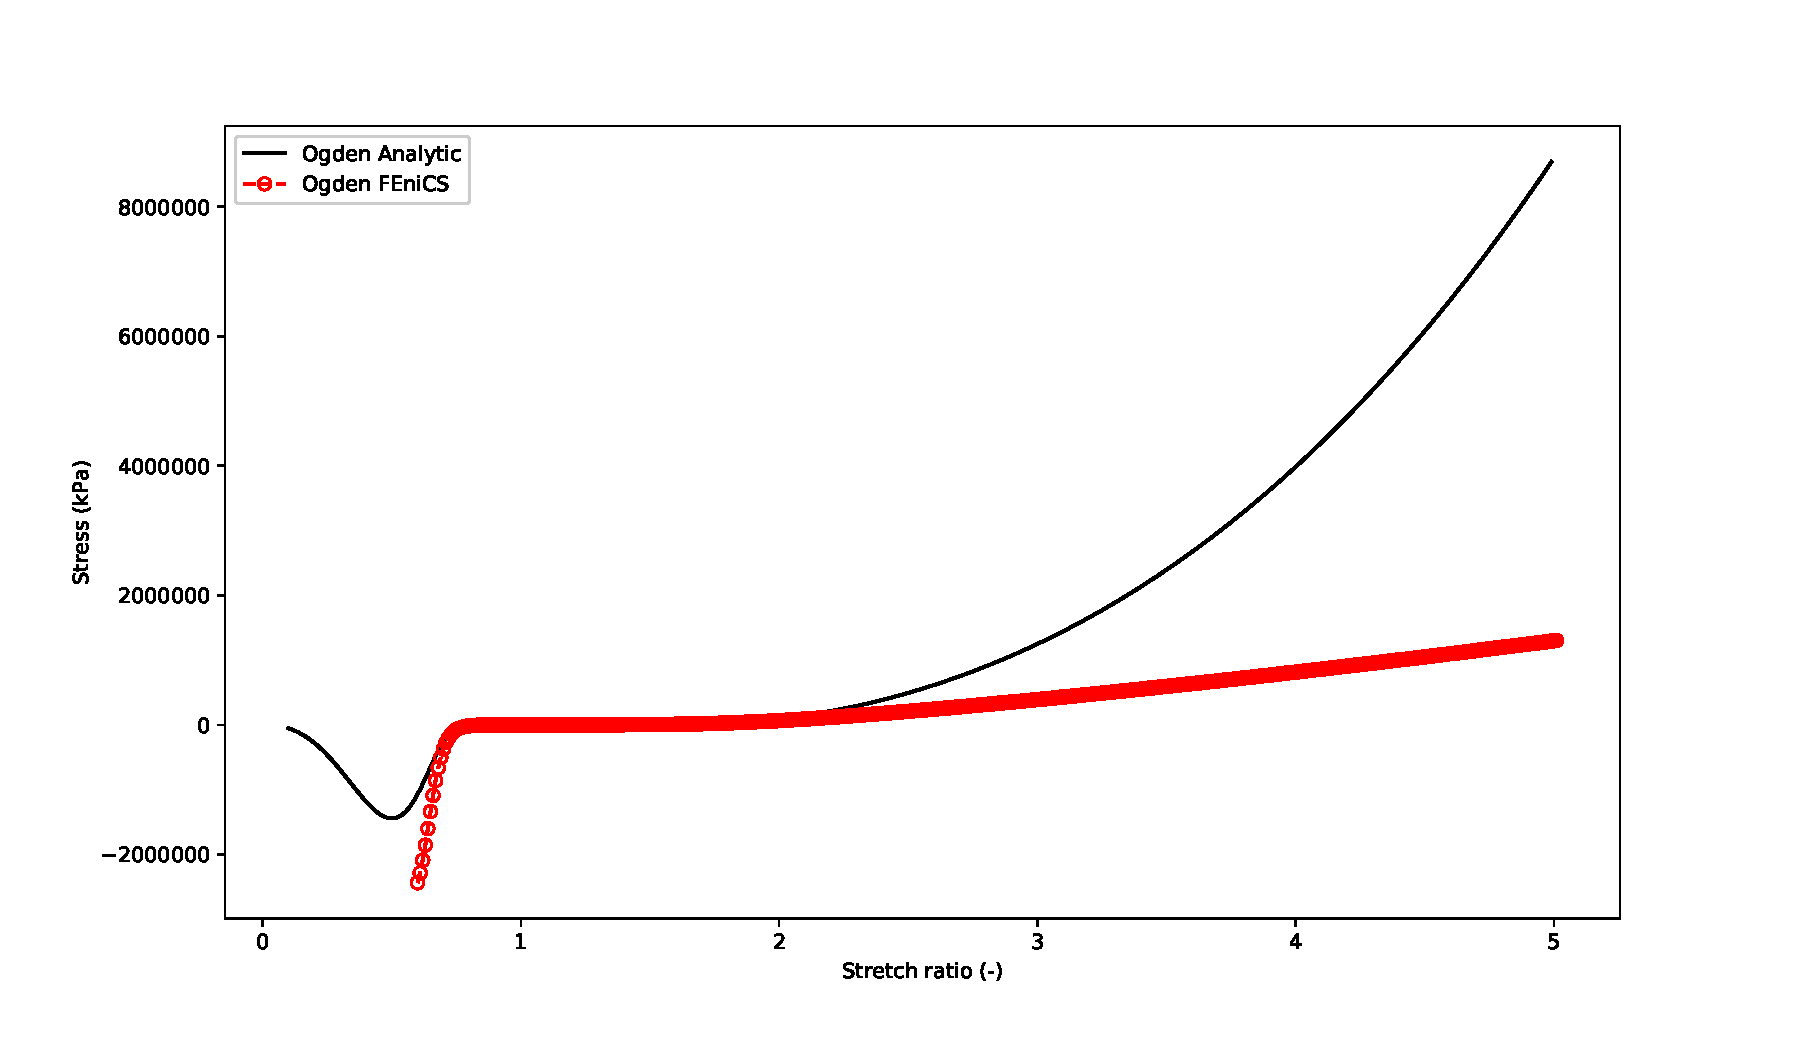
\includegraphics[width=0.25\linewidth, trim =  125 0 125 0]
{Pictures/OgdenCompressibleComparison}}
\\
\subfloat[Neo-Hookean]{
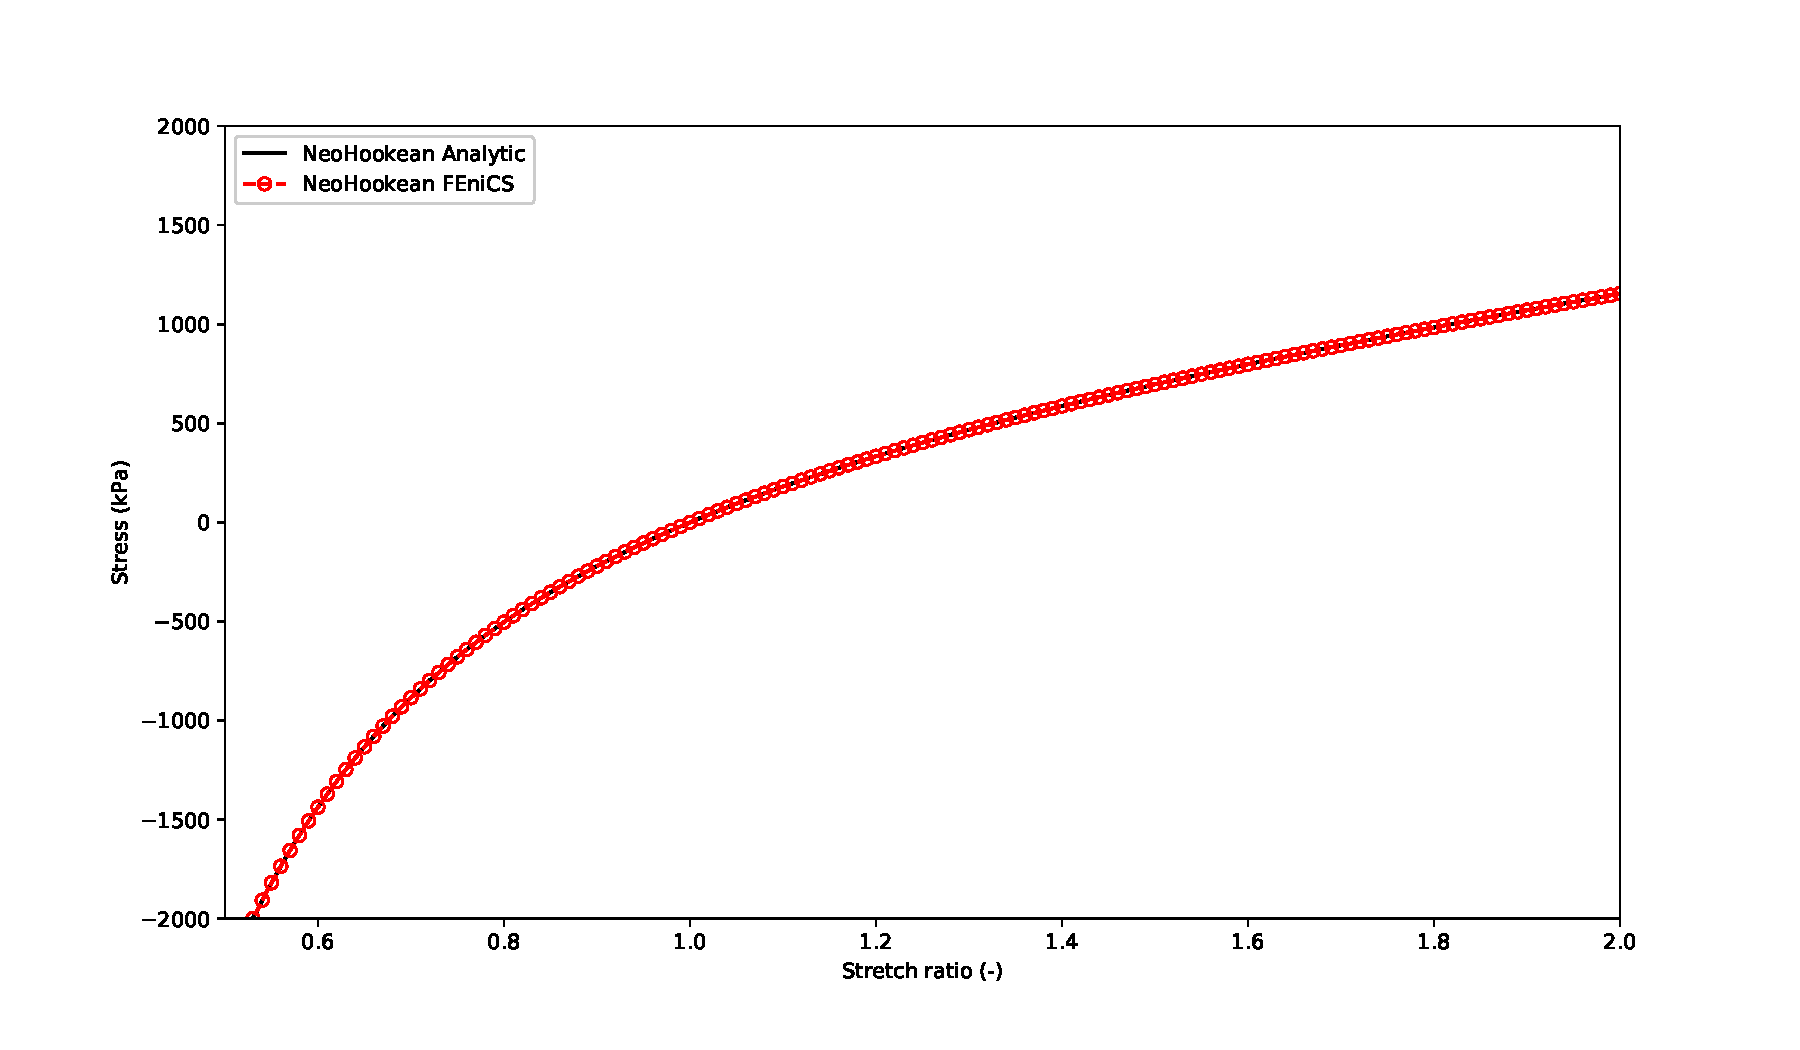
\includegraphics[width=0.25\linewidth, trim = 125 0 125 0]
{Pictures/NeoHookeanCompressibleComparisonZoom}}
\hspace{25mm}
\subfloat[Ogden]{
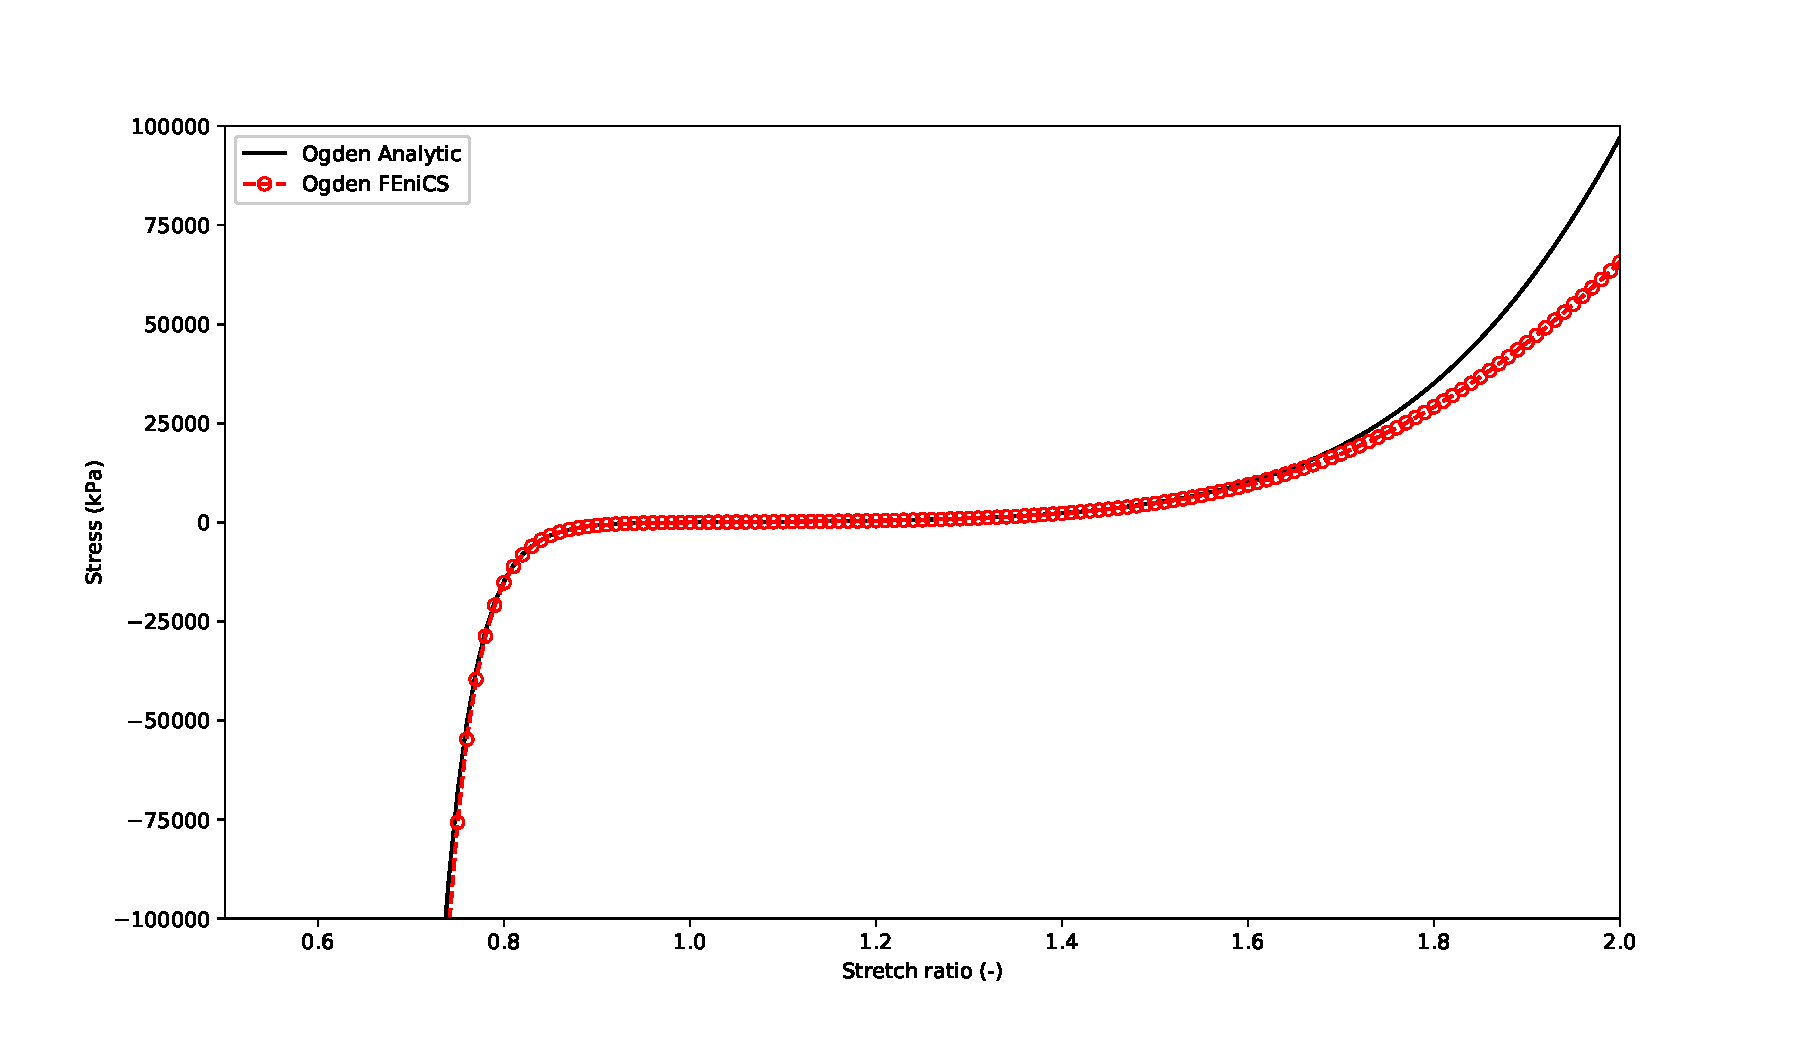
\includegraphics[width=0.25\linewidth, trim = 125 0 125 0]
{Pictures/OgdenCompressibleComparisonZoom}}
\end{figure}
\vfill
\end{columns}
\end{frame}

\begin{frame}
\frametitle{Compressible Ogden Sensitivity}
\begin{figure}
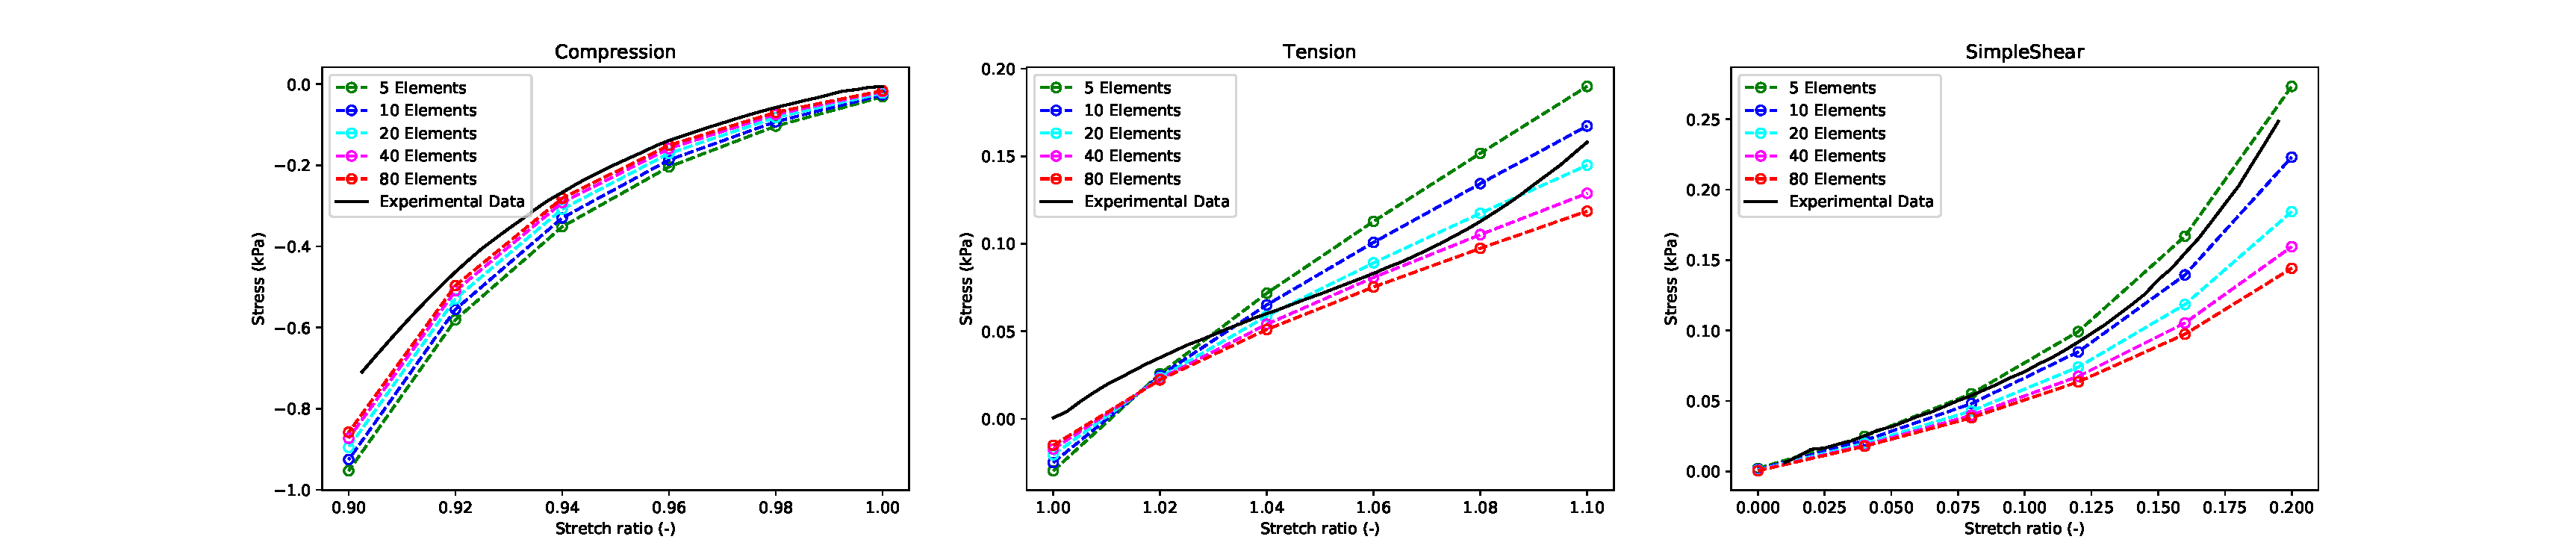
\includegraphics[width=1.0\linewidth, trim =  125 0 125 0]
{Pictures/Sensitivity}
\end{figure}
\end{frame}

\section{Optimization}

\begin{frame}
\frametitle{General}
\begin{itemize}
\item
Optimization first performed in the $\lambda$, $\mu$, and $\alpha$ space
\item
Boundary conditions:\begin{enumerate}
\item
All displacement blocked at the boundaries
\item
Displacement imposed according to the loading case
\end{enumerate}
\item
Compressible Ogden formulation
\item
Optimization using \textit{scipy.optimize.minimize} with the \textit{L-BFGS-B} method
\item
Starting parameters choose according to a review publication (Budday et al.)
\item
Equal weighting of the loading cases in the computation of the cost function
\end{itemize}
\end{frame}

\subsection{Cortex}
\begin{frame}
\frametitle{Cortex - Optimization Settings}
	\begin{table}[h!]
	\centering
		\begin{tabular}{lccc}
		\toprule
		& \textbf{$\lambda (kPa)$} & \textbf{$\mu (kPa)$} & \textbf{$\alpha (-)$}\\
		\midrule
		\textbf{Starting Point} & 10 & 1.43 & -19.0 \\
		\textbf{Optimization Results} & 4.437 & 1.566 & -21.136 \\
		\bottomrule
		\end{tabular}
	\end{table}
\end{frame}

\begin{frame}
\frametitle{Cortex - Cost Function Grid}
\begin{figure}[h!]
\centering
\begin{subfigure}[t]{0.5\linewidth}
\centering
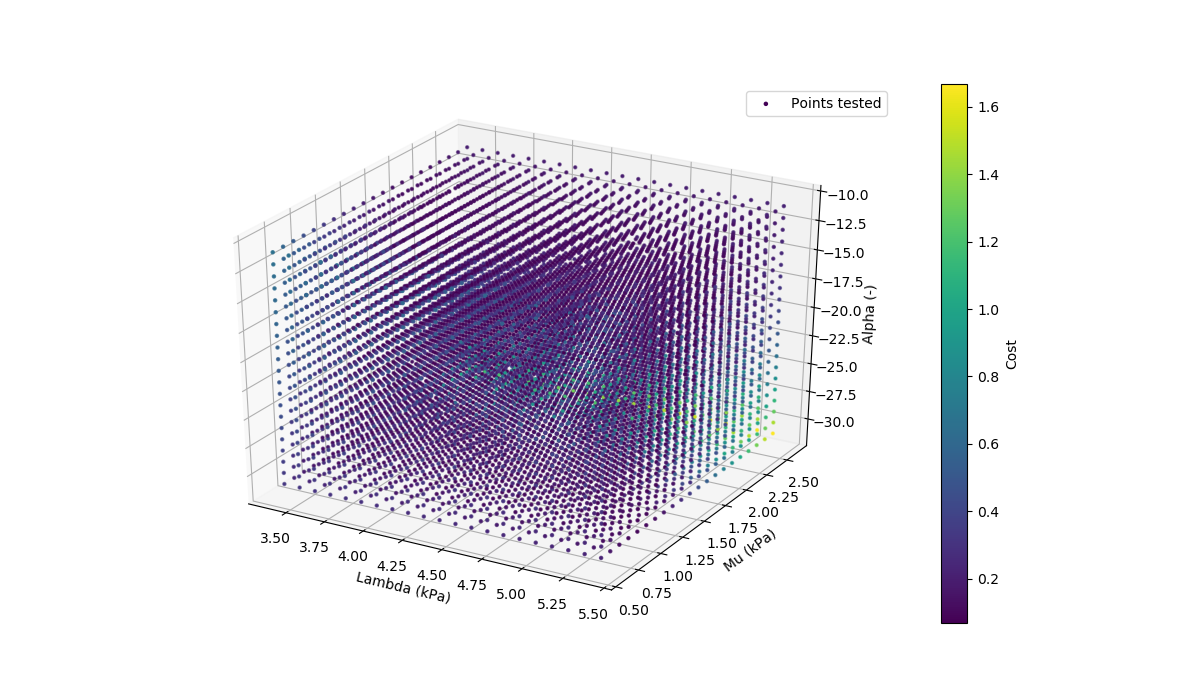
\includegraphics[width = 1.\linewidth, trim = 80 50 50 50]
{Pictures/CortexCompleteGrid}
\caption{Complete grid}
\end{subfigure}%
\begin{subfigure}[t]{0.5\linewidth}
\centering
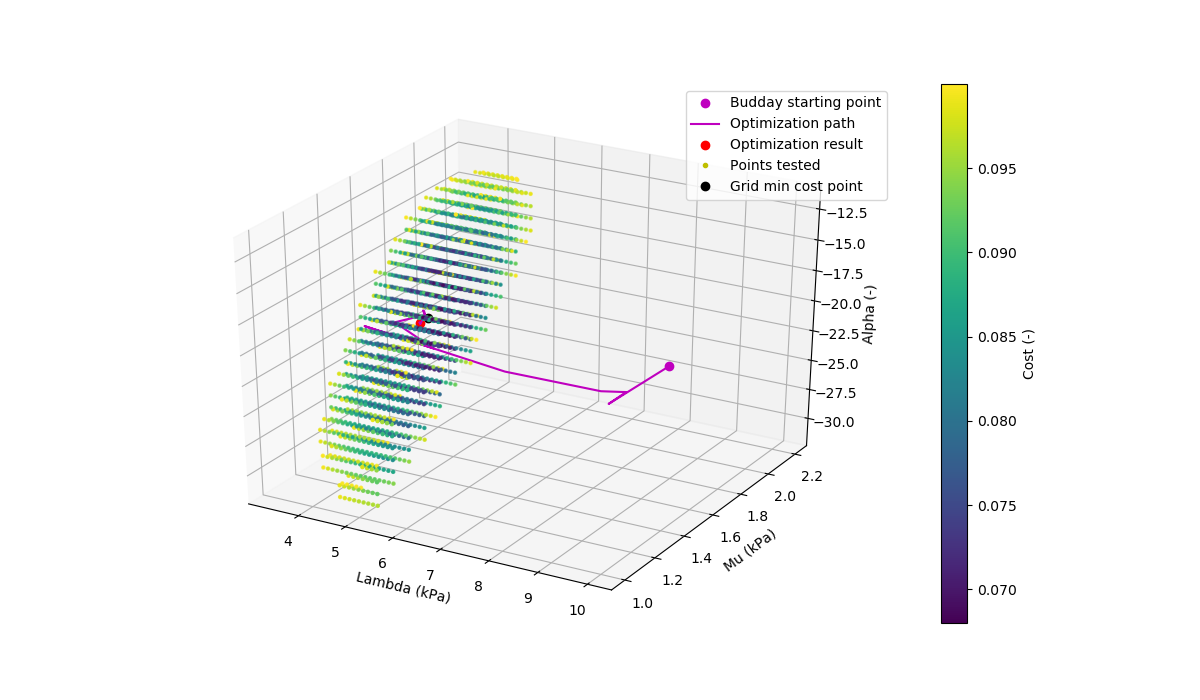
\includegraphics[width = 1.\textwidth, trim = 50 50 80 50]
{Pictures/CortexFilteredGrid}
\caption{Filtered grid}
\end{subfigure}
\caption{Cost function computed points}
\end{figure}
\end{frame}

\begin{frame}
\frametitle{Cortex - Cost Function Grid}
\begin{figure}[h!]
\centering
\begin{subfigure}[t]{0.6\linewidth}
\centering
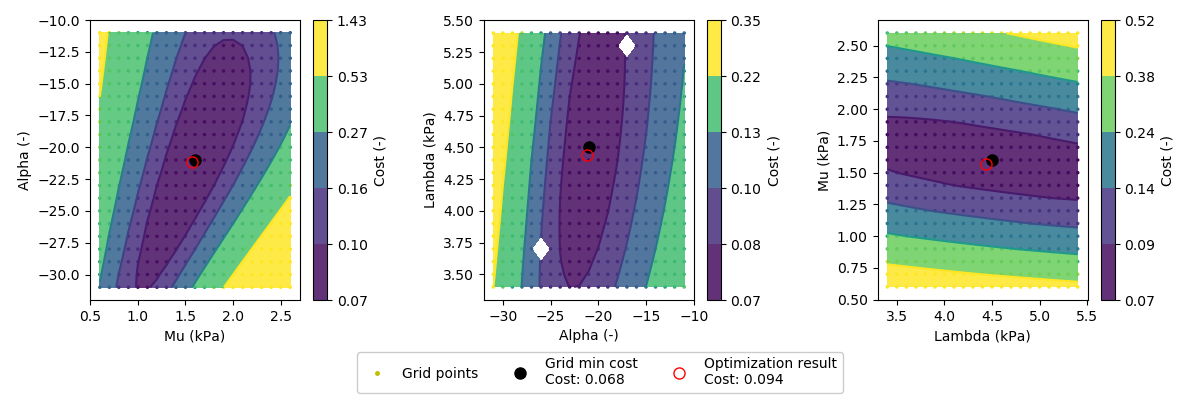
\includegraphics[width = 1.\linewidth, trim = 80 00 50 00]
{Pictures/CortexMinPointProjection}
\caption{2D plot}
\end{subfigure}%
\begin{subfigure}[t]{0.4\linewidth}
\centering
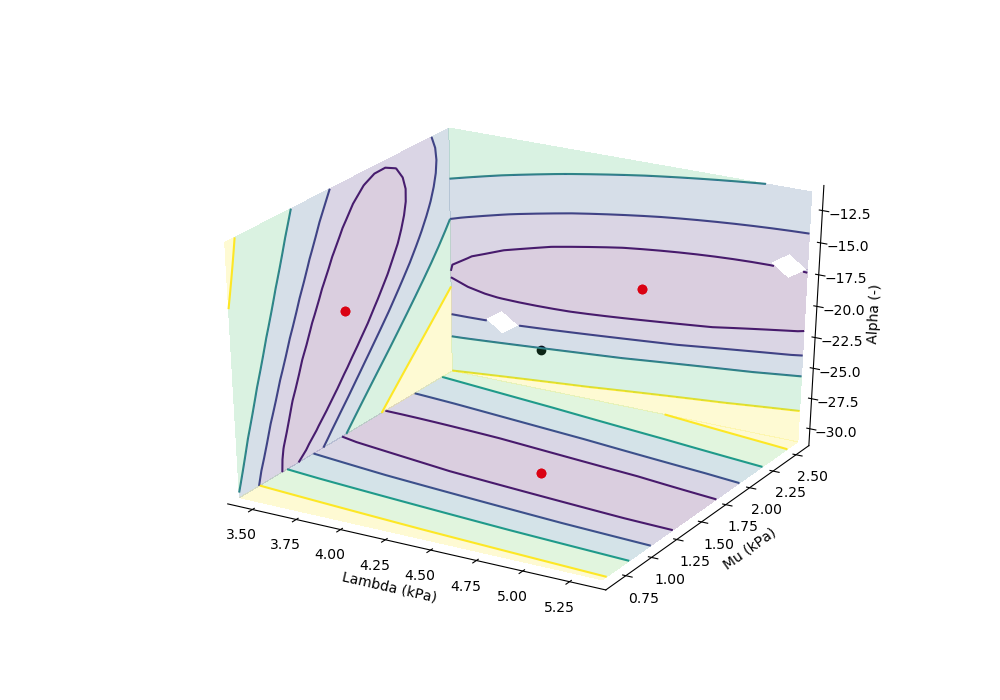
\includegraphics[width = 1.\textwidth, trim = 50 50 80 50]
{Pictures/CortexMinPointProjection3D}
\caption{3D plot}
\end{subfigure}
\caption{Projection of the cost function at the minimum cost point}
\end{figure}
\end{frame}

\subsection{Basal Ganglia}
\begin{frame}
\frametitle{Basal Ganglia - Optimization Settings}
	\begin{table}[h!]
	\centering
		\begin{tabular}{lccc}
		\toprule
		& \textbf{$\lambda (kPa)$} & \textbf{$\mu (kPa)$} & \textbf{$\alpha (-)$}\\
		\midrule
		\textbf{Starting Point} & 10 & 0.7 & -18.7 \\
		\textbf{Optimization Results} & 2.105 & 0.74 & -21.558 \\
		\bottomrule
		\end{tabular}
	\end{table}
\end{frame}

\begin{frame}
\frametitle{Basal Ganglia - Cost Function Grid}
\begin{figure}[h!]
\centering
\begin{subfigure}[t]{0.5\linewidth}
\centering
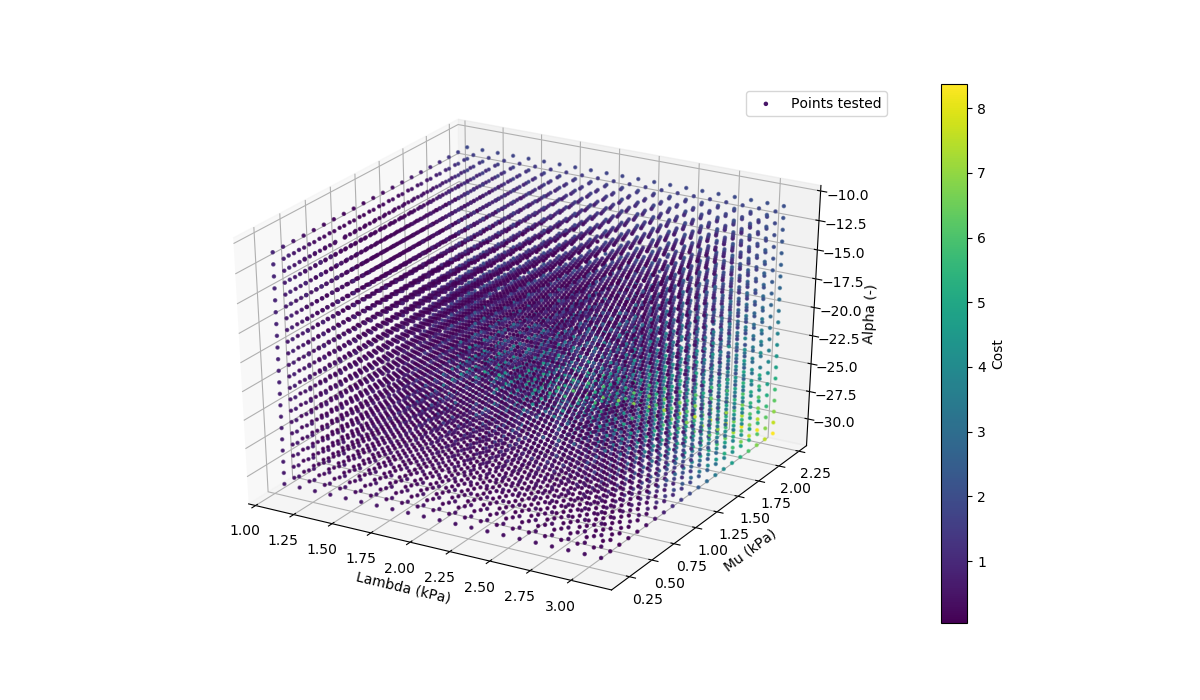
\includegraphics[width = 1.\linewidth, trim = 80 50 50 50]
{Pictures/BasalGangliaCompleteGrid}
\caption{Complete grid}
\end{subfigure}%
\begin{subfigure}[t]{0.5\linewidth}
\centering
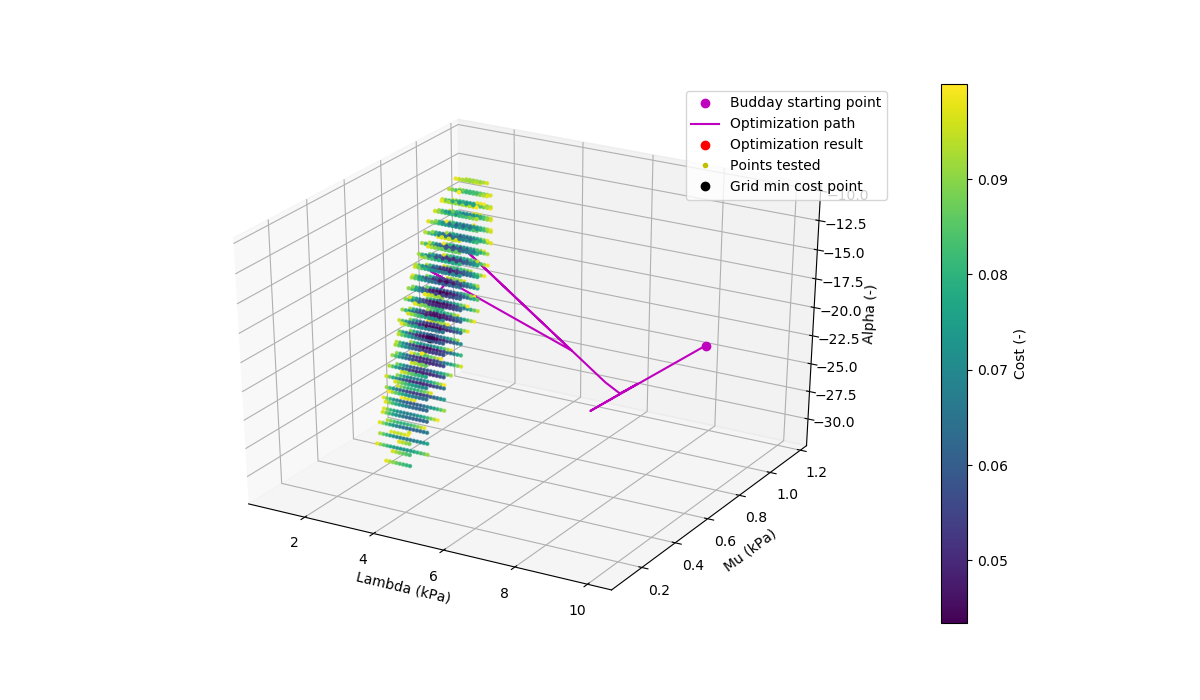
\includegraphics[width = 1.\textwidth, trim = 50 50 80 50]
{Pictures/BasalGangliaFilteredGrid}
\caption{Filtered grid}
\end{subfigure}
\caption{Cost function computed points}
\end{figure}
\end{frame}

\begin{frame}
\frametitle{Basal Ganglia - Cost Function Grid}
\begin{figure}[h!]
\centering
\begin{subfigure}[t]{0.6\linewidth}
\centering
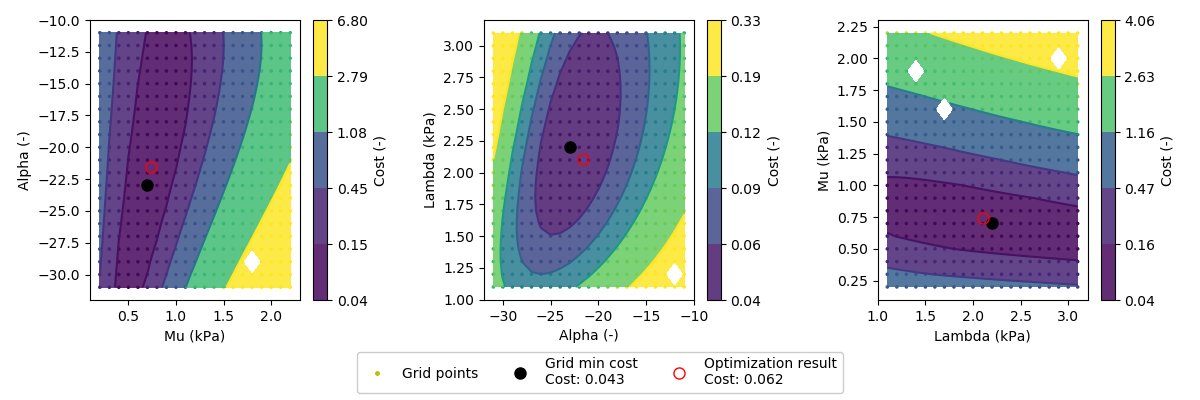
\includegraphics[width = 1.\linewidth, trim = 80 00 50 00]
{Pictures/BasalGangliaMinPointProjection}
\caption{2D plot}
\end{subfigure}%
\begin{subfigure}[t]{0.4\linewidth}
\centering
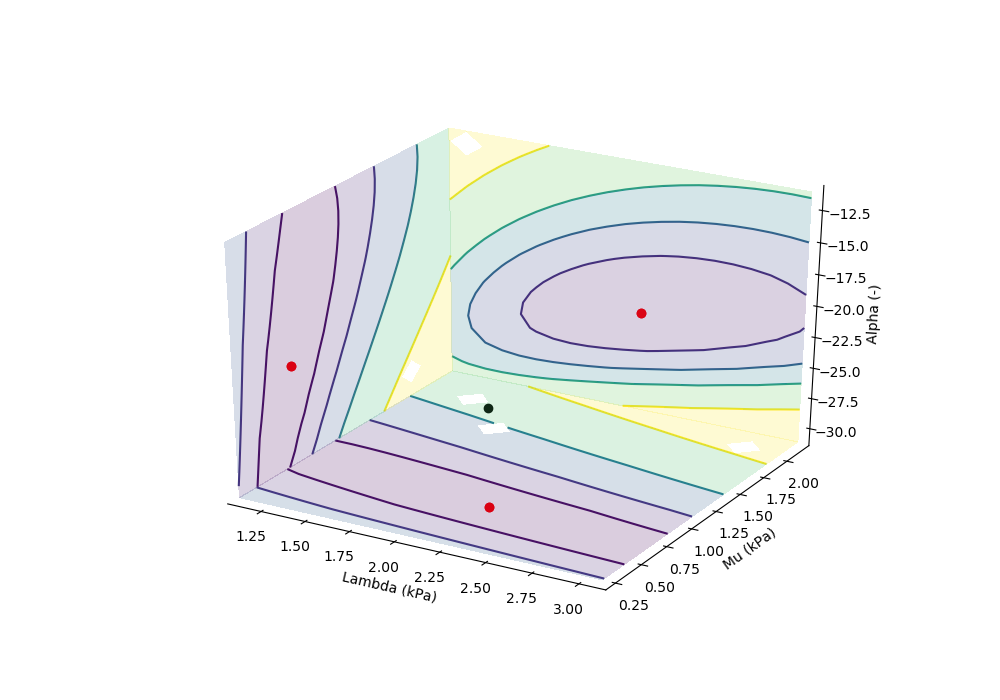
\includegraphics[width = 1.\textwidth, trim = 50 50 80 50]
{Pictures/BasalGangliaMinPointProjection3D}
\caption{3D plot}
\end{subfigure}
\caption{Projection of the cost function at the minimum cost point}
\end{figure}
\end{frame}

\subsection{Corona Radiata}
\begin{frame}
\frametitle{Corona Radiata - Optimization Settings}
	\begin{table}[h!]
	\centering
		\begin{tabular}{lccc}
		\toprule
		& \textbf{$\lambda (kPa)$} & \textbf{$\mu (kPa)$} & \textbf{$\alpha (-)$}\\
		\midrule
		\textbf{Starting Point} & 10 & 0.66 & -24.3 \\
		\textbf{Optimization Results} & 2.057 & 0.659 & -29.398 \\
		\bottomrule
		\end{tabular}
	\end{table}
\end{frame}

\begin{frame}
\frametitle{Corona Radiata - Cost Function Grid}
\begin{figure}[h!]
\centering
\begin{subfigure}[t]{0.5\linewidth}
\centering
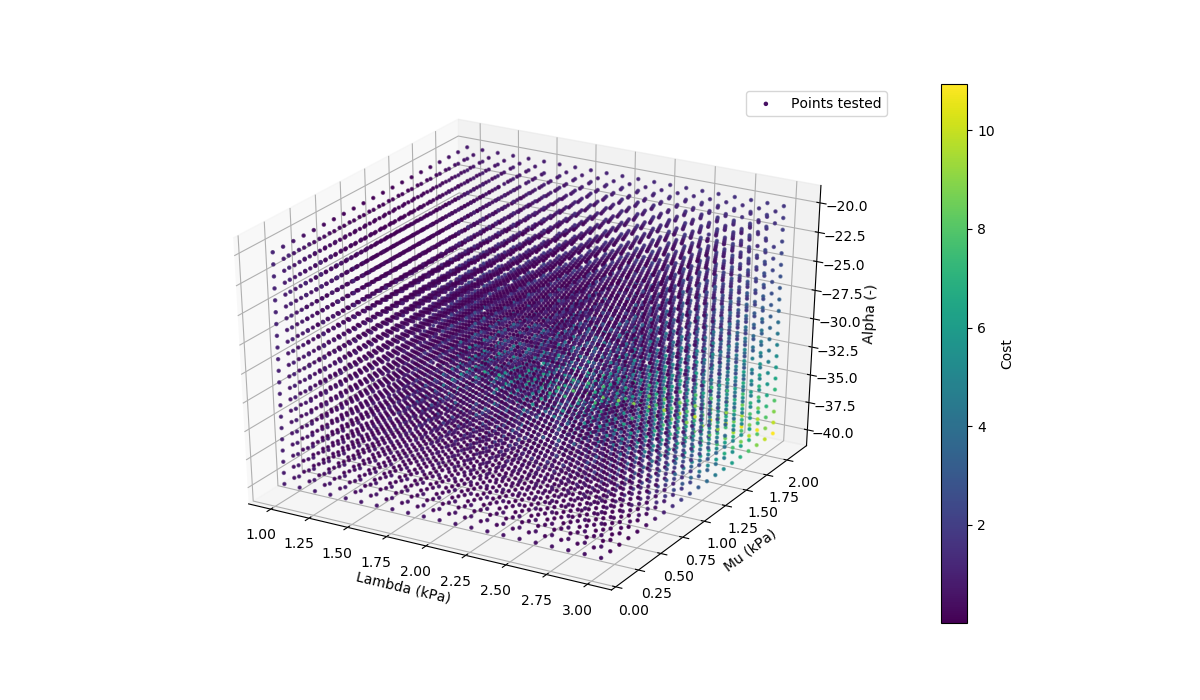
\includegraphics[width = 1.\linewidth, trim = 80 50 50 50]
{Pictures/CoronaRadiataCompleteGrid}
\caption{Complete grid}
\end{subfigure}%
\begin{subfigure}[t]{0.5\linewidth}
\centering
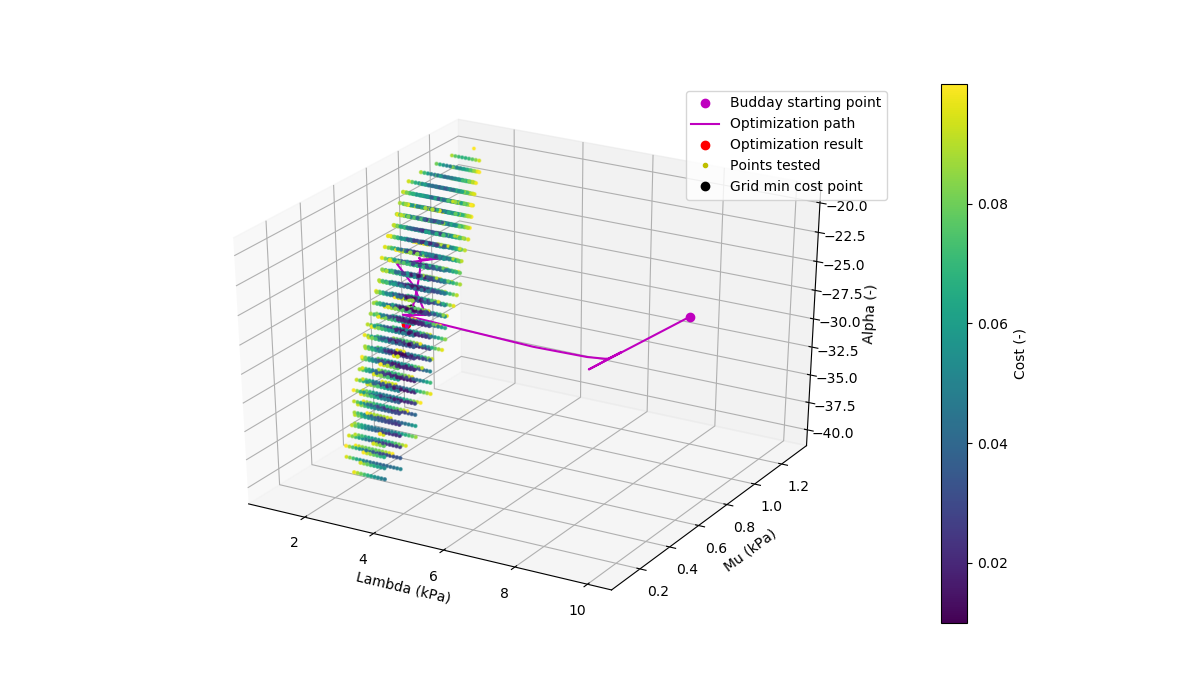
\includegraphics[width = 1.\textwidth, trim = 50 50 80 50]
{Pictures/CoronaRadiataFilteredGrid}
\caption{Filtered grid}
\end{subfigure}
\caption{Cost function computed points}
\end{figure}
\end{frame}

\begin{frame}
\frametitle{Corona Radiata - Cost Function Grid}
\begin{figure}[h!]
\centering
\begin{subfigure}[t]{0.6\linewidth}
\centering
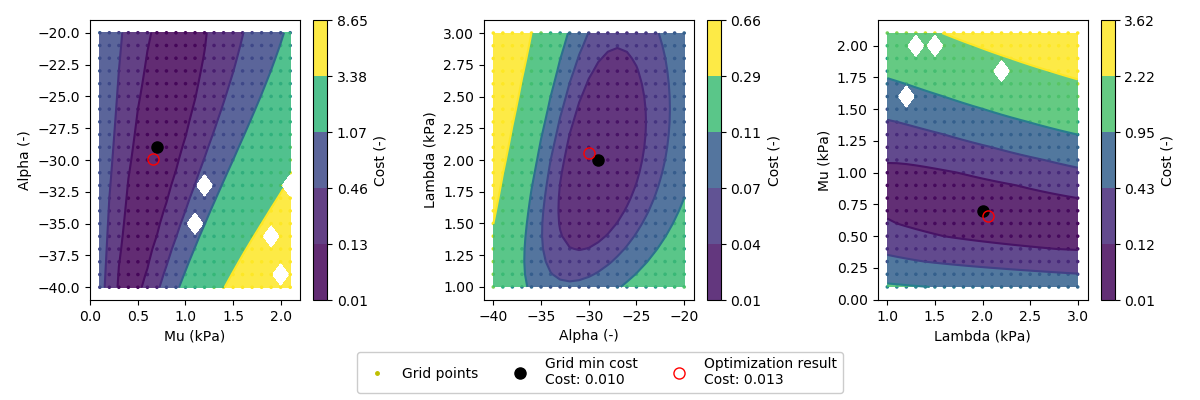
\includegraphics[width = 1.\linewidth, trim = 80 00 50 00]
{Pictures/CoronaRadiataMinPointProjection}
\caption{2D plot}
\end{subfigure}%
\begin{subfigure}[t]{0.4\linewidth}
\centering
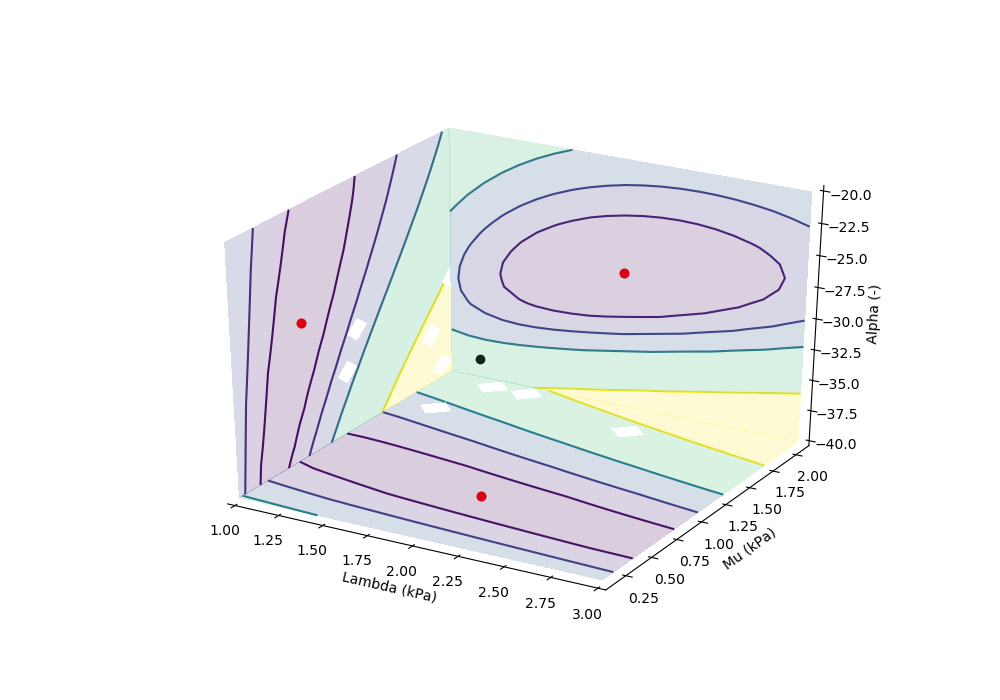
\includegraphics[width = 1.\textwidth, trim = 50 50 80 50]
{Pictures/CoronaRadiataMinPointProjection3D}
\caption{3D plot}
\end{subfigure}
\caption{Projection of the cost function at the minimum cost point}
\end{figure}
\end{frame}

\subsection{Corpus Callosum}
\begin{frame}
\frametitle{Optimization Settings}
	\begin{table}[h!]
	\centering
		\begin{tabular}{lccc}
		\toprule
		& \textbf{$\lambda (kPa)$} & \textbf{$\mu (kPa)$} & \textbf{$\alpha (-)$}\\
		\midrule
		\textbf{Starting Point} & 10 & 0.35 & -25.3 \\
		\textbf{Optimization Results} & 1.219& 0.352 & -30.573 \\
		\bottomrule
		\end{tabular}
	\end{table}
\end{frame}

\begin{frame}
\frametitle{Corpus Callosum - Cost Function Grid}
\begin{figure}[h!]
\centering
\begin{subfigure}[t]{0.5\linewidth}
\centering
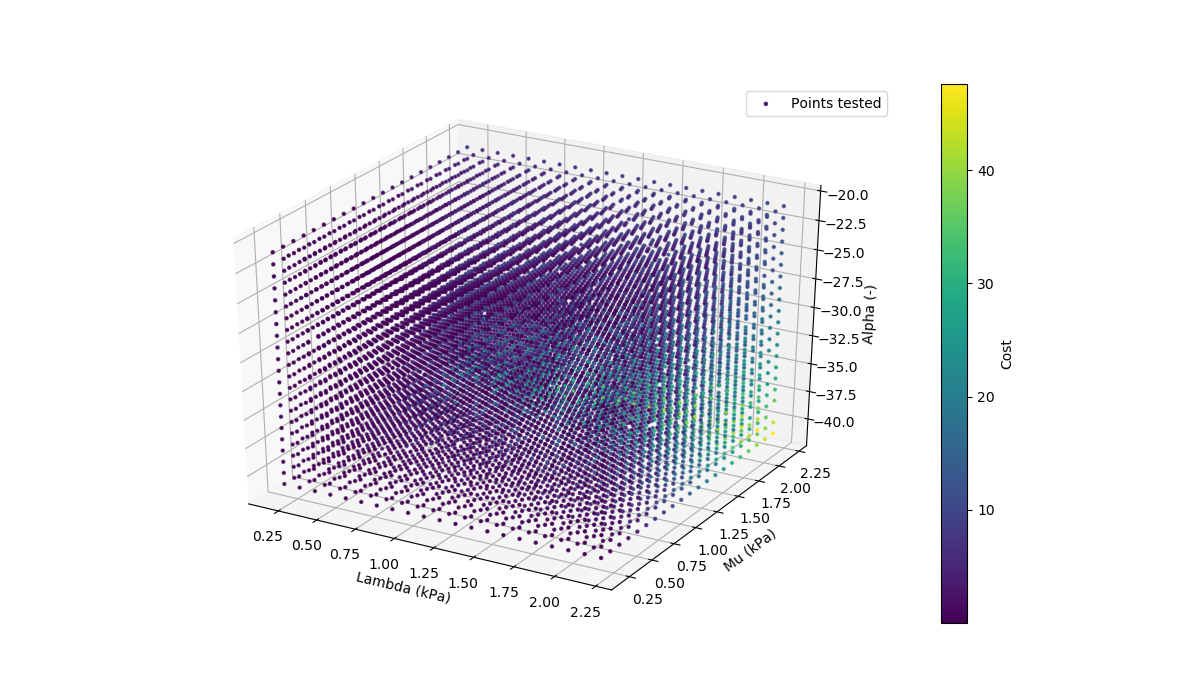
\includegraphics[width = 1.\linewidth, trim = 80 50 50 50]
{Pictures/CorpusCallosumCompleteGrid}
\caption{Complete grid}
\end{subfigure}%
\begin{subfigure}[t]{0.5\linewidth}
\centering
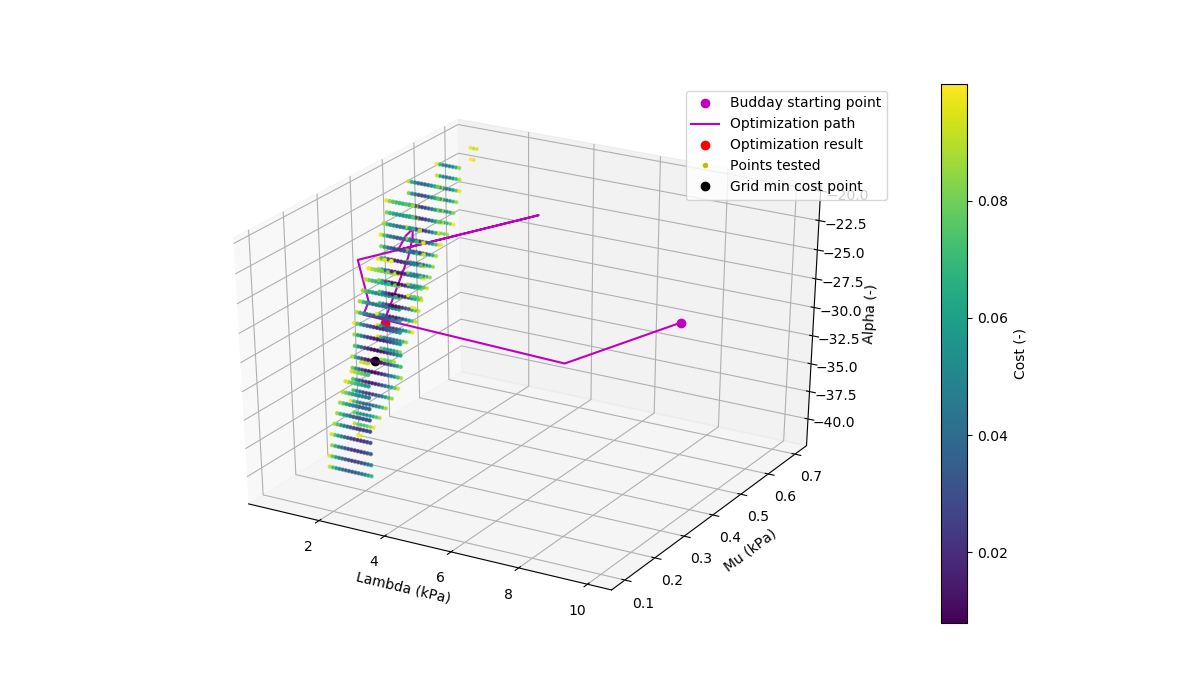
\includegraphics[width = 1.\textwidth, trim = 50 50 80 50]
{Pictures/CorpusCallosumFilteredGrid}
\caption{Filtered grid}
\end{subfigure}
\caption{Cost function computed points}
\end{figure}
\end{frame}

\begin{frame}
\frametitle{Corpus Callosum - Cost Function Grid}
\begin{figure}[h!]
\centering
\begin{subfigure}[t]{0.6\linewidth}
\centering
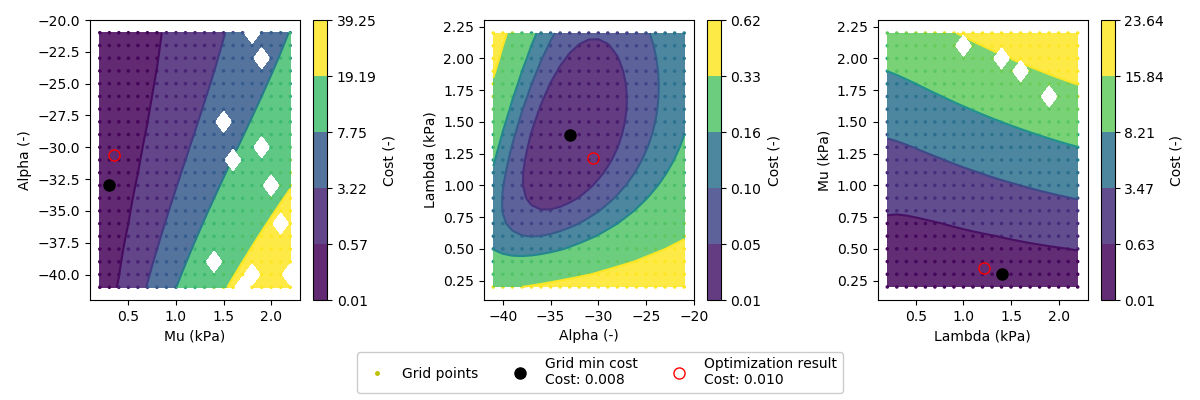
\includegraphics[width = 1.\linewidth, trim = 80 00 50 00]
{Pictures/CorpusCallosumMinPointProjection}
\caption{2D plot}
\end{subfigure}%
\begin{subfigure}[t]{0.4\linewidth}
\centering
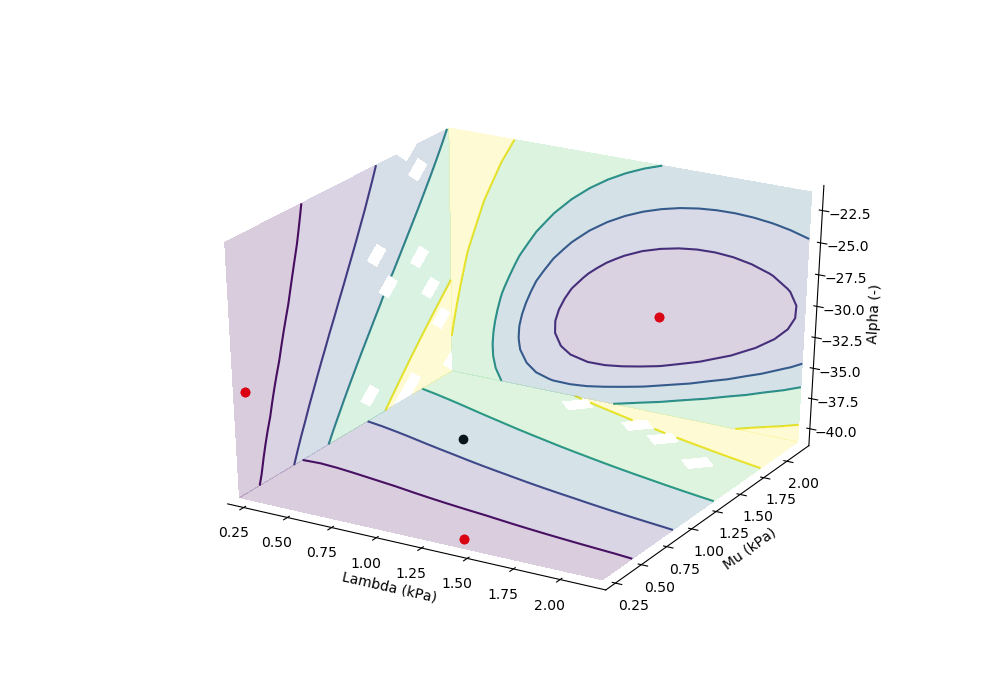
\includegraphics[width = 1.\textwidth, trim = 50 50 80 50]
{Pictures/CorpusCallosumMinPointProjection3D}
\caption{3D plot}
\end{subfigure}
\caption{Projection of the cost function at the minimum cost point}
\end{figure}
\end{frame}

%---------------------------------------------------------------------------------------------------------------------------------------------------
%---------------------------------------------------------------------------------------------------------------------------------------------------
%---------------------------------------------------------------------------------------------------------------------------------------------------
\end{document} 